\documentclass[msc,cs,parskip,leftchapter,logo,twoside,abbrevs,11pt]{infthesis}

\usepackage[square,authoryear]{natbib}
\usepackage{graphicx}
\usepackage{hyperref}
\usepackage{microtype}
\usepackage{eulervm}
\usepackage{color}
\usepackage{listings}
\usepackage{algorithm}
\usepackage{algorithmic}
\usepackage{float}
\usepackage{caption}
\usepackage{subcaption}
\usepackage{lipsum}
\usepackage{verbatimbox}
\usepackage{gnuplottex}
\usepackage{amssymb}
\usepackage{wrapfig}
\usepackage{tikz}
\usetikzlibrary{arrows,automata}

% use eps
\newif\ifpdf
\ifx\pdfoutput\undefined
   \pdffalse
\else
   \pdfoutput=1
   \pdftrue
\fi
\ifpdf
   \usepackage{graphicx}
   \usepackage{epstopdf}
   \DeclareGraphicsRule{.eps}{pdf}{.pdf}{`epstopdf #1`}
   \pdfcompresslevel=9
\else
   \usepackage{graphicx}
\fi

% set colour for listings
\definecolor{mygreen}{rgb}{0,0.6,0}
\definecolor{mygray}{rgb}{0.5,0.5,0.5}
\definecolor{mymauve}{rgb}{0.58,0,0.82}

\lstset{ %
  backgroundcolor=\color{white},   % choose the background color; you must add \usepackage{color} or \usepackage{xcolor}
  basicstyle=\ttfamily,        % the size of the fonts that are used for the code
  breakatwhitespace=false,         % sets if automatic breaks should only happen at whitespace
  breaklines=true,                 % sets automatic line breaking
  captionpos=b,                    % sets the caption-position to bottom
  commentstyle=\color{mygreen},    % comment style
  deletekeywords={...},            % if you want to delete keywords from the given language
  escapeinside={\%*}{*)},          % if you want to add LaTeX within your code
  extendedchars=true,              % lets you use non-ASCII characters; for 8-bits encodings only, does not work with UTF-8
  frame=single,                    % adds a frame around the code
  keepspaces=true,                 % keeps spaces in text, useful for keeping indentation of code (possibly needs columns=flexible)
  keywordstyle=\color{blue},       % keyword style
  language=Java,                 % the language of the code
  morekeywords={def,function,assert,aspect,pointcut,before,transparent,co},
  numbers=left,                    % where to put the line-numbers; possible values are (none, left, right)
  numbersep=5pt,                   % how far the line-numbers are from the code
  numberstyle=\tiny\color{mygray}, % the style that is used for the line-numbers
  rulecolor=\color{black},         % if not set, the frame-color may be changed on line-breaks within not-black text (e.g. comments (green here))
  showspaces=false,                % show spaces everywhere adding particular underscores; it overrides 'showstringspaces'
  showstringspaces=false,          % underline spaces within strings only
  showtabs=false,                  % show tabs within strings adding particular underscores
  stepnumber=1,                    % the step between two line-numbers. If it's 1, each line will be numbered
  stringstyle=\color{mymauve},     % string literal style
  tabsize=4,                       % sets default tabsize to 2 spaces
  title=\lstname                   % show the filename of files included with \lstinputlisting; also try caption instead of title
}

% include subsubsections in toc
\setcounter{secnumdepth}{5}
\setcounter{tocdepth}{5}

% Change font to palatino
% Euler for math | Palatino for rm | Helvetica for ss | Courier for tt
\renewcommand{\rmdefault}{pplx} % rm
\linespread{1.05}        % Palatino needs more leading

\title{Dynamic Parallelism Detection for the HotSpot\texttrademark Java Virtual Machine}
\author{Christopher Edward Atkin-Granville}

\abstract{Contemporary computers are highly based around highly parallel architectures through chip multiprocessors, instruction-level parallelism and graphics processing units with potentially thousands of cores. Despite this, many popular programs are based around a sequential programming paradigm. This project investigates the use of the Graal compiler infrastructure in order to dynamically profile running programs within the Java Virtual Machine and determine which hot loops are good candidates for automatic parallelism transformations, possibly JIT recompilation to an OpenCL target.

We consider two main approaches to trace collection: exact approaches and probabilistic approaches.}


\begin{document}
	\begin{preliminary}
		\maketitle
		\begin{acknowledgements}
		I wish to thank my supervisors, Dr. Christophe Dubach and Dr. Bj\"{o}rn Franke for their insightful and valuable contributions to the project.

		Also in need of thanks are my parents, Sandra and Ian who have supported me throughout my entire University career.
		\end{acknowledgements}
		\standarddeclaration
		\dedication{To my grandfather, Leslie.}
		\tableofcontents
		\listoffigures
		%\listofalgorithms
	\end{preliminary}

	\chapter{Introduction} \label{chp:introduction}
In this chapter, some background to the problem of parallelism and parallel expression is presented. Some alternative approaches to dynamic detection are covered (\ie, alternative parallel expression techniques), with a critical analysis of their strengths and merits. Lastly, a brief overview of the outline of this dissertation is presented.

\section{Background} \label{sec:introduction/background}
Ever since the introduction of the first microprocessors in the early 1970s, there has been a trend within the microprocessor industry affectionately called Moore's Law. Although not a law in the proper scientific sense (rather, it is more of an observation of the behaviour of the industry), it does accurately describe the trend of the number of transistors which can be placed in a given area\footnote{Which is emphatically \textit{not} the idea that processor speed doubles every 18 months - which is a common misconception. Moore's Law is also applicable to other VLSI products, such as memory.}. The trend so far has been that this number double every 18 months. Altogether, Moore's Law successfully described the behaviour of the semiconductor industry until roughly five years ago.

\section{Golden Age} \label{sec:introduction/golden-age}
During this time of rapid advancement, programmers had to expend very little effort in order to improve performance of their programs on newer hardware. In the best-case scenario, literally no change was required whatsoever - not even a recompilation of the program. The underlying hardware was improving, and when one combines this fact with the separation of concern between user-level applications and the underlying hardware (i.e., the abstraction layer that compilers introduce, with a special focus on ISA abstraction) meant that developers could simply urge their users to buy new hardware for a performance improvement.

In a slightly less-than-idea scenario, the higher transistor counts being allowed would allow semiconductor designers to add new features to the `base' instruction set of their choice - for example on x86 there have been several additions over the years (MMX, 3DNow!, SSE, PAE, x86-64 etc). In these cases, programmers would simply need to recompile their programs with a compiler that would take advantage of the new extensions. Platforms supporting just-in-time (JIT) compilation such as Java, C\# etc would need to replace existing virtual machines (VMs) with ones capable of using the new instruction sets.

In many ways, this time could be seen as a golden age of computer architecture. Transistors were cheap and plentiful and the promise was always there that next year transistors would be even cheaper and more plentiful. Semiconductor manufacturers started experimenting with radical new designs (not all of which were successful, for example Intel's NetBurst which promised speeds of up to 10GHz by, amongst other techniques, involved utilising an extremely long pipeline). Consumers were confident that a new machine would be significantly faster than the machine they purchased a mere 12 months prior. Enabled by the new-found performance of processors, application developers would start to introduce many new layers of abstraction (and indirection), which would allow for safer, stabler programs to be written using high-level languages such as Ruby, Python, Perl and PHP. These extremely-high-level (EHL) languages (sometimes called scripting languages) commonly sacrificed execution speed for programmer ease of use, safely, new features and other such advantages. Indeed, this phenomenon even became widespread in lower-level languages via Java and C\#, both of which introduced a virtual machine between the application and the hardware. In many cases, these virtual machines were specifically designed (at least initially) for the languages for which they were designed (in that they were not initially designed to be `language agnostic'), meaning they may have allowed features that are difficult to implement lower in the stack. For example, the Java Virtual Machine (JVM) includes opcodes such as \texttt{invokespecial} (which calls a special class method), \texttt{instanceof} and other such codes specifically designed for an object-oriented language\footnote{There is currently an effort to add new instructions to the JVM designed to ease execution of languages with non-object-oriented paradigms}. These features are enabled via high-performance processors, and would likely not exist (or certainly, not be mainstream) without these processors.

\section{Cheating the System} \label{sec:introduction/cheating}
However, these increases cannot occur indefinitely. There exists not only a fundamental lower-bound on the size of an individual transistor (as a result of quantum tunnelling), but also the extent to which contemporary techniques can provide performance improvements. For example, many common processors exploit instruction-level parallelism (ILP) by executing several instructions at the same time - pipelining. This is achieved by effectively duplicating many stages of the pipeline and the supporting infrastructure. Besides the standard issues with pipelining (data, control and structural hazards spoiling issue flow, multi-cycle instructions spoiling commit flow and the like which can be solved via trace caches, as done in the Pentium 4), there exists a larger problem. As the degree to which ILP is exploited in a processor increases, the complexity of the supporting infrastructure increases combinatorially. Hence, this is clearly not the `silver bullet' which ILP was once thought to be. The extent to which current processors exploit ILP are not likely to increase significantly in the next several years, barring a revolutionary breakthrough in processor manufacturing, ILP detection/exploitation etc.

About a decade ago, it was a commonly held belief that the path to improving processor performance was to make a single-core processor increasingly powerful, through a combination of higher clock speeds (which manifested itself as the so-called `Megahertz War') and architectural improvements. Although this did come true to an extent (eventually culminating in the 3.8GHz Intel Pentium 4), this period did not yield the kind of performance that was expected (see above). The main reason for this was a simple one - transistors with higher switching frequencies produce more heat. This, when combined with the fact that Moore's Law would allow higher transistor counts per unit area meant that around 2006 to 2007 manufacturers were unable to improve performance much more simply through increasing the clockspeed.

\section{Hello, Parallelism} \label{sec:introduction/parallelism}
There existed no simple solution to this problem. For decades developers were used to having to expend little to no effort to realise potentially significant performance improvements. The solution that industry converged upon was that of parallelism - to improve performance not by increasing the performance of a single processor, but to provide many processors each of which are slightly slower when taken individually. When combined together (with a multi-threaded program), the culmination of these processors would be more performant than a single processor could ever be.

Parallelism (and concurrency) was not a new idea. For decades parallelism had been used for the most compute-intensive problems (such as ray tracing and scientific computing). These kinds of problems are usually `embarrassingly parallel' - each unit of work is totally independent from all other pieces of work. Example of this include ray-tracing, where each ray can be simulated independently; rasterisation, where each pixel can be computed in parallel and distributed scientific problems such as SETI@Home. Indeed, concurrency has been part of developers standard toolkit for many years since the advent of GUIs. In Java developers commonly use helper classes such as \texttt{SwingWorker} to run compute-intensive GUI tasks in a thread independent from UI event processing in order to prevent the UI `hanging' when performing long-running computations.

However the level of parallelism present in most applications is fairly superficial. Even using tools such as \texttt{SwingWorker} does not introduce a significant level of parallelism. For example, imagine a button that invokes a \texttt{SwingWorker} which executes a loop for many iterations. Although that loop is running on a different thread, that loop is \textit{still} executing sequentially. A significant performance improvement could be realised if the developer had introduced structures and  processes that allow the loop to be executed in parallel; unfortunately these transformations are non-trivial and hence are usually not performed.

Regardless of the main reason that parallelism hasn't been introduced to any significant degree in programs (i.e., there was not a pressing need to), there are still many barriers to introducing parallelism. The main problem is likely that most developers simply do not have the required education or experience to do so. Parallelism and concurrency introduces many subtle timing errors that appear transiently. Scheduling algorithms are usually non-deterministic, which makes reasoning about them (either formally or informally) difficult. The behaviour of multi-threaded programs can change with varying number of processors.

\section{Parallelist Approaches} \label{sec:introduction/parallelist}
One solution to this problem that has been advocated by many theoretical computer scientists and language designers is to switch language paradigm to functional languages such as Haskell and Erlang. Languages and systems of this class do have significant advantages - both theoretical and applied - over more conventional paradigms. Purely functional languages have first-class, referentially-transparent functions which can be easily reasoned about by both the user and the compiler. However, here are two main disadvantages to this approach. Although it is the most optimal from a theoretical perspective (and mainstream switching to a functional language would bring many benefits, not just increased parallelism), it would require rewriting existing programs in a functional language. Moreover, most developers do not have experience with functional languages - and are not, unfortunately, willing to learn. It is not a problem of technology - more one of education.

Moving more towards the practical side of things, there are two main alternatives. The first is to use language-level constructs which are built into the semantics of the language. There has been some work in this area, and they usually focus on extending existing languages with parallel semantics. These additions usually provide language-level constructs for message passing, parallel loop construction, barriers and other such low-level parallelism primitives. Although there are many such research languages (Click-5, Chapel, X10 etc), there exists no commonly used language supporting these features. There are also some hybrid languages, such as Lime which are backwards compatible with existing infrastructures. The advantages of these languages is that because they support parallelism primitives intrinsically, reasoning and inference (both by humans and in an automated fashion) is much easier than it is for other languages. Adding support for parallelism at the language level also, depending on the level of abstraction used, implies tying a language to a particular parallel paradigm (or set of paradigms). If a language implements low-level constructs instead of higher-level constructs (similar to algorithmic skeletons except at the language level), then the user has to implement many commonly used operations manually, leading to bugs and inconsistencies between implementations. The education issue is also present with language-level constructs. Despite these disadvantages, some progress has been made in this area by Microsoft with PLINQ (Parallel Language Integrated Query), which is a declarative extension to CLI languages. PLINQ is successful because it requires little to no changes from standard LINQ - this is the ideal scenario in many cases (although note that PLINQ is not a general-purpose solution).

A more pragmatic approach to language-level constructs is a library-based approach such as POSIX Threads (Pthreads), OpenMP and OpenMPI. Pthreads is an implementation of the POSIX (\textit{Portable Operating System Interface}) standard regarding threads and is therefore compatible with a wide variety of hardware and operating systems (including some non-POSIX compliant systems such as Windows). OpenMP is a library for C, C++ and Fortran for shared-memory programming, although it is commonly used to implement parallel loops (i.e., work sharing). OpenMPI is similar to OpenMP with the exception that it is designed for distributed-memory programming instead. The advantage of a library-based approach is that users can `mix-and-match' between different libraries - for example, a user can use both OpenMP and OpenMPI within the same program. However, many of the libraries require significant low-level knowledge of parallelism, and are not particularly user friendly.

To illustrate the substantial difficulties of adding parallel semantics to existing programs with sequential semantics, let us consider the challenges programmers face when using parallel features in programming languages, such as threads. Mutual exclusion is, currently, the most widely adopted parallel programming paradigm, as it is the easiest to use (although it does not nessecarily offer the greatest performance; nevertheless it can offer performance greater than that of sequential programs). Some common issues include \citep{Fraser04,Herlihy1993,ppls}:

\begin{itemize} \label{lst:parallelhard}
	\item \textbf{Deadlock}: where two or more threads are waiting on each other to finish before continuing 
	
	\item \textbf{Livelock}: similar to deadlock, except that the threads are changing state yet not achieving work
	
	\item \textbf{Priority inversion}: when a thread with high priority is pre-empted by a thread with a lower priority
	
	\item \textbf{Race conditions}: the result of two or more threads attempt to access the same resource(s) at the same time, leading to non-deterministic behaviour
\end{itemize}

There have been some attempts to mitigate these issues (\eg \citet{Liu2011}), but they have not yet been widely adopted.

Many web-scale companies (Facebook, Google, Yahoo! etc) have large datasets that require (offline) processing and are now using parallel infrastructures such as Hadoop (MapReduce) to support this computation. Such infrastructures are similar to library-based solutions except that they also provide management solutions and other such features. Hadoop, along with its sister projects HDFS, Hive and HBase, provide an entirely framework for programming, executing, distributing and managing parallel applications. An `all-in-one' solution such as Hadoop is extremely attractive simply because it provides everything one needs to set up distributed/parallel applications. The disadvantage is that, in general, such frameworks are only suited to a single kind of parallel framework. In the case of Hadoop, it can only support MapReduce-based computations. In other words, all computations that are not based around a MapReduce model are incompatible with Hadoop. Additionally, such frameworks typically require a large number of resources in order to be effective (Hadoop may actually \emph{reduce} performance of computations if the number of processors is small), although that disadvantage is not inherent to MapReduce-style computations.

Perhaps the `holy grail' of parallelism is the idea of an auto-parallelising compiler. In other words, a compiler that can infer enough information about the semantics of the program in order to apply transformations that convert a program with sequential semantics into one with parallel semantics. This approach sounds extremely attractive, as it would not require (ideally) any effort on the behalf of the programmer; despite this there are significant disadvantages. Firstly, given the scope and context of contemporary common languages (C, C++, Objective-C, C\#, Java), applying compile-time transformations to add highly context-sensitive parallel semantics is likely in intractable problem. The reason for this is that, with current compiler technology, it is not possible to infer enough information regarding the semantics and syntax of the languages to reason about them. To illustrate this point, even when additional parallel semantics are added to existing languages (with sequential semantics), loops may still not be easily parallelisable because of pointer aliasing For example, imagine a function that returns an array of values which cannot be determined at compile-time. If that array is then used to index another array (say in a vector addition), reasoning about the parallel semantics of that vector addition are intractable at compile-time.

The last kind of parallelism is hardware-supported parallelism through constructs such as transactional memory (\textit{TM}). TM solutions have the advantage of being easily programmable (to the extent that they are as easy as marking a method as \textit{synchronized}, similar to how Java's monitors operate i.e., coarse-grained parallelism) whilst retaining the performance of fine-grained parallelism. The disadvantage of this approach is that high-performance TM architectures are reliant on hardware support (although software-based approaches do exist, they typically exhibit significantly lower performance characteristics than a similar hardware-based approach). Additionally, simply adding TM into a program does not add parallel semantics to a program with sequential semantics - constructs that allow e.g. threads to be created still need to be added. TM can rather be seen as of a way to make parallel programming easier, not a complete solution.

Transactional memory is, in effect, an optimistic memory model in that multiple threads attempt several transactions at the same time, and any conflicting writes are \emph{rolled fine}. The final operation to be performed in a transaction is a \textit{commit} operation - where the changes are recognised permanently in global state. However, unlike database management systems which are concerned with the ACID properties \citep[p.~14]{DatabasesBook}:

\begin{itemize}
	\item \textbf{Atomicity}: the `all-or-nothing' execution of transactions
	\item \textbf{Consistency}: no transaction can move global state from a consistent state to an inconsistent state
	\item \textbf{Isolation}: the fact that each transaction must appear to be executed as if no other transaction is executing at the same time
	\item \textbf{Durability}: the condition that the effect on global state of the transaction must never be lost once the transaction is complete
\end{itemize}

However, transactional memory when used in the context of computer systems (TM can be implemented in both hardware and software, but as the semantics are the same we shall consider only transactional memory `in the large'), we are principally concerned with only atomicity and isolation, as we assume that changes to memory do not need to be durable (memory operations are transient) \citep{Marshall2005}.

Another way of utilising hardware support in parallelism is to make use of low-level constructs such as compare-and-swap, test-and-set (and test-and-test-and-set) and so on. These mechanisms are very simple, but they allow programmers to implement more complicated and sophisticated parallelism constructs using them. For example, the test-and-test-and-set operation can be used to implement locks in the following way:

\begin{lstlisting}[caption=Pseudocode for a test-and-set atomic operation and its use,label=lst:testandset]
boolean function test-and-set(boolean v) {
    < boolean initial = v;
      v = true;
      return initial;
    >  }
// usage of test-and-set
lock_t lock = false;
co [int i = 1 to n] {
    while (something) {
        // test lock before test-and-set(lock)
        // via short-circuit evaluation
        // this is to avoid trashing the cache
        while (lock || test-and-set(lock)) ;
     
        critical-section();
        lock = false;
        non-critical-section();
    }
}
\end{lstlisting}

{\small Note that any code within $<$ and $>$ occurs atomically, and the \texttt{co} notation refers to $n$ threads executing the block in parallel.}

However, such approaches are equivalent to using a low-level language such as assembly or C to write a modern application - they are simply too low-level for programmers and are highly error prone.

It is interesting to note that languages with theoretical, rather than pragmatic, roots display excellent characteristics for automatic parallelisation. For example, functional languages display characteristics such as referential transparency. Referential transparency is the property that a function is composed entirely of \textit{pure functions} - functions that do not modify global state. The advantage of this, along with the other properties of functional languages, is that it allows the compiler to reason about the program. Functions that display referential transparency lend themselves to easy automatic parallelisation.

Indeed, this idea of higher-level languages displaying good parallelisation characteristics extends to languages other than just functional languages. Many declarative languages (where the programmer describes \emph{what} he/she wants to happen, in a sense without expressing control flow) lend themselves to automatic parallelisation, because they allow the compiler (or interpreter) to reason about the language. Declarative languages are semantically a `purer expression' of computation in the sense that they do not contain implementation details, which allows this reasoning by the compiler.

\section{Language Semantics and Compiler Reasoning} \label{sec:introduction/reasoning}
Referential transparency is advantageous for parallelisation because it limits shared state. The reason that the techniques listed above such as semaphores, mutexes and so on is to limit concurrent access to shared state variables. As referential transparency specifically disallows shared state, the advantages are clear. To give a concrete example of this, consider the following code, noting that function $f$ is declared as referentially transparent:

\begin{lstlisting}[caption=Example of a referentially transparent function,label=lst:reftrans]
int transparent function f(int x, int y) {
    return x * y;
}

results = int array[10000][10000]

for int i = 0 to 10000 {
    for int j = 0 to 10000 {
        results[i][j] = f(i, j)
    }
}
\end{lstlisting}

Because $f$ has been declared as transparent, the compiler can perform aggressive optimisations - \eg for $p$ processors, computing $\frac{10000}{p}$ iterations of the outer loop on each processor. It must be emphasised that the specific runtime configuration is not important - it is up to the compiler or runtime to determine the appropriate execution strategy. In theory, the compiler or runtime could even execute the loops on a more specialised device, such as a GPU.

So far in this chapter we have justified the use of declarative languages over imperative/procedural languages for parallelisation because they allow the compiler to reason about the semantics of the language \citep{PeytonJones2011}. But what does it mean for a compiler to `reason' about a language? To answer this, let us consider some examples.

Consider the following SQL statement:

\begin{lstlisting}[language=SQL,caption=Sample SQL query,label=lst:sql]
SELECT
    username, firstname, lastname
FROM
    Users
WHERE
    id = 3
\end{lstlisting}

As we know, SQL is a declarative language. The user has \emph{no} control over the way that the SQL compiler/optimiser/interpreter/runtime executes the query, and this is precisely the power that declarative languages offer. Research has shown that optimistic optimistic compilers for declarative languages can, in some cases, out-perform hand-tuned C code \citep{Anderson2013,Mainland2013}.

Declarative languages have already successfully been applied to several different area of parallel computing \citep{Orchard2010,Grossman2011,Holk2011}.

% language-level
% libraries
% infrastructures (Hadoop)
% auto-threading compilers
% hardware assistance

\section{Outline} \label{sec:introduction/outline}
This dissertation is split into several chapters.

Chapter \ref{chp:introduction} outlines the problem background and context, including an overview of the current most common approaches to parallelism expression. Chapter \ref{chp:related} describes the previous work both the areas of dynamic parallelism detection and parallelising compilers/runtime systems. Chapter \ref{chp:graal} is an outline of the Graal compiler infrastucture, the main tool used in the project. Chapter \ref{chp:instrumentation} provides an overview of the possible approaches to instrumenting Java bytecode where appropriate. Chapter \ref{chp:runtime} introduces the approaches to trace storage from both theoretical and practical perspectives. A software engineering-based overview of the approaches used is also included. Chapter \ref{chp:methodology} describes the experimental design, configuration and other parameters. Chapter \ref{chp:results} presents the findings and a critical analysis of the work. The last chapter, chapter \ref{chp:conclusion} draws final conclusions about the work, and suggests possible areas of future work in this area.
	\chapter{Related Work} \label{chp:related}
The idea of an automatic parallelising compiler is not a particularly new one, and indeed has been the focus of much research since the dawn of structured programming with Fortran \citep{Backus1979}.

In this chapter, some background of both parallelising compilers and parallelism detection will be presented. The areas have a rich and full history spanning many decades (indeed, the objective of automatic parallelising compilers has been sought for many years), so this is a somewhat brief introduction; only the recent major results are considered.

\section{Dynamic Parallelism and Parallelism Extraction} \label{sec:related/compilers}
Runtime systems with this capacity are advantageous because they require no access to the source code. In \citeyear{Yang2011}, \citet{Yang2011} introduced one of the main advances in the field, \textit{Dynamic Binary Parallelisation}. It requires no access to the source code, and instead operates only using object code. The mechanism through which it operates is by detecting hot loops -- loops where the program spends a majority of execution time -- and parallelises them, executing the parallel versions speculatively. This speculation is likely the cause of the inefficiencies of their approach - using 256 cores they achieved a somewhat negligible performance improvement of just 4.5 times, and the reason for this is likely hazards spoiling the speculation frequently, which requires expensive rollbacks. However, one of the advantages of the approach presented in this dissertation is that it does not require the use of speculative execution - a loop is only executed if it can be proven to contain no inter-iteration dependencies.

The main difference between \citeauthor{Yang2011}'s work and the work outlined here is the nature of the dynamic detection. \citeauthor{Yang2011} used dynamic trace analysis, which can only identify the hot loops within a program, and not whether the iterations within those loops have dependencies. The work presented in this dissertation \emph{does} determine whether there are inter-loop dependencies, therefore the use of speculative execution is not required. Although we have not yet done so, the addition of hot-loop detection would be a trivial addition to our framework.

\citet{Wang2009} used a technique called \textit{backwards slicing} \citep{Weiser} in order to preserve essential dependence and data flow. The advantage of an approach based on slicing is that it can detect parallelism regardless of the granularity. This is in contrast to the work presented in this dissertation which can currently only detect parallelism at a loop-level. \citet{Wang2009} represents the first work in the area of dynamic parallelisation using a splicing-based approach. An approach based on slicing can determine different `sections' of a program (such as blocks, if-then-else statements and so on) which can be executed in parallel, allowing the runtime system to execute in parallel. The algorithms in this paper are speculative - if a dependency is detected at runtime, the pararallelisation for both blocks must be rolled back and instead executed in parallel. \citeauthor{Wang2009} present a new set of algorithms for extraction of parallelism. These algorithms can:

\begin{itemize}
        \item Determine loop-unrolling factors to expose maximum parallelism
        \item Identify backwards slices for hot regions
        \item Exploit speculation in program slicing
        \item Group the large number of slices
\end{itemize}

The approach to slicing is based on static analysis, with an additional speculative execution model. The speculations performed are:

\begin{itemize}
        \item \textbf{Memory speculation}: memory dependencies on operations that occur infrequently ($<$0.1\% according to profiling) are ignored
        \item \textbf{Control speculation}: control flow edges that are rarely executed ($<$0.5\%) are cut
        \item \textbf{Branch prediction}: highly identifiable branches are cut
\end{itemize}

Performance of the system was adequate, with a roughly 3x performance improvement with unlimited threads, and 1.8x parallelism with four threads. The major disadvantage to this approach is that the complexity of the slicing algorithms increases exponentially with the length of each slice, meaning that only relatively small slices can be detected and hence parallelised.

An alternative approach was taken by \citet{Ketterlin}. Their technique `raises' binary code into an intermediate form (similar to how Graal converts bytecode, see chapter \ref{chp:graal} for more details), and then applies a well-known parallelising transformation.

\citet{Dong} present a framework that is capable of dynamic parallelisation for general-purpose graphics processing cards (GPGPU technology). GPGPU technology allows the large number of processors in GPGPUs to be used by the user for executing large programs. These processors are simpler than the general-purpose cores found in normal CPUs, and so there are some constraints placed on programs.

The framework presented takes a binary loop body and generates IR from it, similar to both Graal and \citet{Ketterlin}. Then, the IR is combined with statically-determined loop information to perform static analysis on the code. A translator is then used to transform the sequential C code into C code that can be executed in parallel using CUDA. The framework is advantageous in that it can parallelise multiple nested loops, increasing performance for many applications. However, it relies on static analysis for dependency analysis, and it does not use speculation to increase performance. However, despite these limitations, the results are acceptable, showing performance improvements of 18x for large matrix multiplication, and betwen 15x and 32x for MRI scan analysis. Importantly, such a framework -- or indeed, any framework based around executing using GPGPUs -- has a efficacy lower-bound placed on it by using a GPGPU. Transferring data to a GPU for execution has large overhead, with a large startup cost. The result of this is that only large loops should be effectively parallelised using GPGPUs; if this is not the case then an otherwise effective parallelisation framework may result in performance decreases.

Another approach taken is the one taken by \citet{Tournavitis2009}. Instead of applying more traditional algorithms to the problem, \citeauthor{Tournavitis2009} instead use machine learning, specifically Support Vector Machines. The aims and philosophy behind the paper are similar to this project: \citeauthor{Tournavitis2009} argue that static parallelism detection has failed because there is not enough information available at compile-time - the same reasoning that this project assumes.

The paper presents an approach to auto-parallelisation based around a combined profile of statically and dynamically generated metadata, which is then fed into a pre-trained support vector machine (SVM). This SVM provides information about how the loop should be parallelised. This approach is significant because it compromised three approaches - static analysis, dynamic analysis and machine learning. The paper presents result of up to 96\% that of hand-tuned OpenMP code, which shows clearly that the use of machine learning in compilers can result in significant performance advantages. 

\citet{Rogers2005} presents a dynamic parallelisation framework within the Jikes Research Virtual Machine (RVM), an alternative JVM implementation. The authors used static analysis in order to prove dependencies, and the framework  applies parallelisation techniques based around extended array SSA form. Loops are detected via back edges in the control-flow graph. Unfortunately, the transformations added Java threads as a parallelisation primitive, which have high spawn overheads. As a result, in many cases the speepup after parallelisation was lower than that of the pre-transformation program. Parallel speedups ranged from 0.7\% to 3.7\%, but the separate overhead of applying and executing the transformation meant that execution times were higher. This demonstrates the need for both efficient instrumentation as well as efficient run-time transformation capabilities.

\section{Instrumentation} \label{sec:related/instrumentation}
Although in this dissertation we consider dynamic instrumentation, a significant amount of work is available in the literature describing \emph{static instrumentation}. Static instrumentation modifies bytecode directly at load-time and is `dumb' in the sense that it is possible to only gain access to information available statically. This is unlike dynamic instrumentation which has access to the full control flow graph and other such information.

Here, we consider some of the various different approaches to static instrumentation.

\subsection{Bytecode Instrumentation} \label{sec:instrumentation/bytecode-instr}
The first approach uses so-called \textit{bytecode instrumentation} (BCI) - that is, modifying the bytecode directly, either at compile-time or runtime. This approach is advantageous in that arbitrary commands can be inserted, and is only subject to the limitations of the bytecode format. In this sense, arbitrary functionality can be inserted into \texttt{.class} files. However, it is complex (requiring advanced knowledge of the JVM and bytecode formats), as well as being difficult to use. Graal already performs a lot of the work that would be required with this kind of approach, in that it detects control flow and memory dependencies from bytecode. Such systems require a large degree of programmer effort.

	\subsubsection{Java Agents} \label{sec:instrumentation/bytecode-instr/agents}
	At the heart of BCI is the idea of Java Agents \citep{javaagents}. In order to understand them, however, one must first understand some details of the Java platform.

	Unlike some other languages (for example, C and C++\footnote{Although note that C and C++ \emph{also} support dynamic linking}), Java is a dynamically linked language. That is to say that the various different libraries (JARs) that Java programs used are linked at run-time, rather than compile-time. The advantage to this approach is that it allows distributables to be smaller in size (recall Java Network Launching Protocol, a method for launching (and therefore, distributing) Java applications over the Internet). The disadvantage to this approach is that it can lead to `dependency hell', although through the combination of versioning metadata in JARs and the extreme backwards compatability mantra in Java, this is not currently a significant issue.

	There are three main class loaders in Java:

	\begin{itemize}
		\item The system class loader loads the classes found in the \texttt{java.lang} package
		
		\item Any extensions to Java are loaded via the extension loader

		\item JARs found within the class path are loaded with the lowest precedence, these include the majority of user-level libraries
	\end{itemize}

	Java Agents manipulate class files at load-time, through the \texttt{java.lang.instrument} package. The package defines the \texttt{ClassFileTransformer} interface, which provides implementations of class transformers. An advantage of this approach is that since Java Agents are included in the core Java package, developers wishing to use the framework would not need to download any additional libraries or frameworks (\ie, Graal).
	
	This mechanism allows agents to dynamically alter the bytecode at load-time, a kind of polymorphism. Such transformations could be utilised in modifying the bytecode of, \eg array accesses in loops to include calls to instrumentation.

	There are several different libraries which provide an abstraction layer for such bytecode transformations. The following sections describe various different libraries that could be used (or use themselves) for agent-based bytecode instrumentation.

		\subsubsection{ASM} \label{sec:instrumentation/bytecode-instr/asm}
		Despite Java Agents providing the capability to manipulate raw Java bytecode (indeed, the bytecode is made available as a \texttt{byte} array), performing such transformations is difficult and awkward. For this reason, there exists many different libraries for manipulating Java bytecode, ObjectWeb ASM being one of them.

                ASM \citep{Bruneton2002} is a simple-to-use bytecode manipulation library, itself written in Java. It uses a high-level abstraction for the bytecode, which is advantageous because it allows developers to remain unconcerned with the specifics of control flow analysis, dependency analysis and other such concerns.

                Although now common, when ASM was first developed it was considered particularly innovative because it allowed the use of the visitor pattern \citep[p.~331]{Gamma1995} for traversing bytecode. The visitor pattern `allows for one or more operations to be applied to a set of objects at runtime, decoupling the operations from the object structure' \citep{McDonald2008}. The advantage to this approach is that it allows a user to walk a serialized object graph \emph{without} de-serialising it or defining large numbers of classes (for reference, an alternative to ASM for bytecode generation, BECL \citep{ApacheBECL} contains 270 classes for representing each bytecode). Additionally, it allows users to also reconstruct a modified version of the graph (in ASM, graphs are immutable).

                Several well-known existing projects use ASM already for bytecode generation, including the Groovy programming language \citep{GroovyDocs}.

                ASM was selected as a possible alternative for this project for several reasons. Firstly, its visitor pattern-based approach to bytecode generation/modification is high-level and easily understandable. It also has high performance, being a factor of 12 more performance than BECL for serialisation/deserialisation, and a factor of 35 times more performance than BECL for computing maximum stack frame sizes. ASM is also superior to BECL for performing modifications, although with a significantly lower margin of just a factor of four.

                The reason for this performance improvement is likely the way ASM and BECL are designed. BECL follows a strict, classical interpretation of object-oriented design principles. Although `good' software design, it is well known that object models have considerable overhead.

                \subsubsection{Javassist} \label{sec:instrumentation/alt-instr/bytecode-instr/javassist}
                Javassist \citep{Chiba1998} is similar to ASM in that it is also a library for manipulating bytecode, but its method of operation is significantly different. It allows for run-time polymorphism, by dynamically switching implementation of classes at run-time.

                There are also additional libraries for manipulating Java bytecode, but due to their features (or lack of), they were not considered for this project.

        \subsection{Aspect-Oriented Programming} \label{sec:instrumentation/alt-instr/aop}
        Aspect-Oriented Programming (AOP) \citep{Kiczales1997} is another dialect of object-oriented programming that aims to significantly increase separation of concern within programs, so that programs are more loosely coupled. AOP is a direct descendent from object-oriented programming as well as reflection. Reflection allows programmers to dynamically introspect classes at run-time; changing values and so on. AOP takes this to another level, by allowing so-called \textit{advice} to be specified (essentially the additional behaviour to be added) and added to \textit{join points}, which are arbitrary points of control flow within the program.

        When combined, aspect-oriented systems add these behaviours to the program in question at compile-time through a process called \textit{weaving}.

        To illustrate this concept, consider the problem of logging method calls. In traditional systems, at each function/method definition the programmer would need to add specific logging code:

        \begin{lstlisting}[caption=Traditional use of advice in programs,label=lst:tradadvice]
def function name(...) {
    if (DEBUG)
        println("function called at " + time());

    // other statements
}\end{lstlisting}

        This behaviour is called an \textit{aspect} (an area of a program which may be repeated several times which is unrelated to the purpose of the program). If the behaviour is to change (\eg for example, changing the call to \texttt{date()} to a call to \texttt{time()} instead), each method declaration must be changed manually - a time consuming and potentially error-prone task.

        Instead, the use of aspects allows the programmer to remove this functionality, and combine a pointcut and advice into an \textit{aspect}:

        \begin{lstlisting}[caption=AOP-based advice equivalent to listing \ref{lst:tradadvice},label=lst:aopadvice]
def aspect TraceMethods {
    def pointcut method-call: execution.in(*)
        and not(flow.in(this));

    before method-call {
        println("function called at " + time());
    }
}\end{lstlisting}

        Although that from a software engineering perspective this is clearly a superior solution (as it decreases coupling, increases reuse, increases separation of concern), the use of aspects has not been widely adopted. There are several likely causes for this, such as:

        \begin{itemize}
                \item \textbf{Lack of education}: widespread adoption of new programming constructs requires that the average programmer can understand the feature without in-depth education in the model. AOP is somewhat counter to intuitive definitions of imperative or procedural languages, which hampers their adoption
                
                \item \textbf{Lack of language support}: no widely adopted programming language comes with AOP included, or with an AOP library included in the standard library. Standard licensing issues also apply to third-party additions (\eg GPLv2/3 differences)
                
                \item \textbf{Unclear flow control}: perhaps the single largest issue with AOP. As noted by \citet{Constantinides2004}, aspects introduce effectively unconditional branches into code, mimicking the use of \texttt{goto} which \citeauthor{Dijkstra1968} famously considered harmful \citep{Dijkstra1968}
                
                \item \textbf{Unintended consequences}: defining aspects incorrectly can lead to incorrect (global) state, \eg renaming methods and so on. If a team of developers are unaware of each other's modifications at weave-time, there may unintended consequences and subtle (or substantial) bugs introduced
        \end{itemize}

        \subsection{AspectJ/ABC} \label{sec:instrumentation/aop/aspectj}
        AspectJ \citep{Kiczales2001} is an extension to the Java language that adds aspect-oriented features. It is a project of the Eclipse Foundation (of Eclipse IDE fame). The usage of AOP within Java is a somewhat natural extension as aspects can be seen as the modularisation of behaviour (concerns) over several classes - and not to forget that AOP was originally developed as an extension to object-oriented languages.

                \subsubsection{Array and Loop Pointcuts} \label{sec:instrumentation/aop/aspectj/arrayloop}
                However, the limitations of the AspectJ join-point model are somewhat obvious for this project. To be specific, `vanilla' AspectJ cannot define point cuts for neither array accesses or loops - a combination of which would be required for this project. In addition, the vanilla AspectJ implementation is not particularly extensible, which means that defining new point-cuts is somewhat difficult.

                There is, however, an implementation of AspectJ which \emph{is} designed to be more extensible and compatible (mostly) with the original AspectJ implementation - abc, the AspectBench Compiler for AspectJ \citep{Allan2005}.

                Although abc itself does not include point-cuts for either array access or loops, there exists two projects which, if combined, could offer the required features for this project.

                LoopsAJ \citep{Harbulot2005} is an extension to abc that adds a loop join point. This is not a trivial addition - when loops are compiled, they are compiled to forms that lose loop semantics (and instead use \texttt{goto} instructions). There are several forms that a loop can take, and a significant proportion of \citeauthor{Harbulot2005}'s work is in the identification of loops from the bytecode.

                For array access, the ArrayPT project \citep{Chen2007} adds additional array access capabilities to abc. Although the included point cut does include array access, it is somewhat limited and cannot determine either the index, nor the value to be stored. ArrayPT adds these capabilities to abc. ArrayPT defines two new point cuts, \texttt{arrayset(signature)} and \texttt{arrayget(signature)}. ArrayPT relies on the \texttt{invokevirtual} bytecode in the JVM.

                It is anticipated that, if these projects are combined, it would present a feasible approach to instrumentation.

        \subsection{Hybrid Models} \label{sec:instrumentation/hybrid}
                \subsubsection{DiSL} \label{sec:instrumentation/hybrid/disl}
                Recently, there has been renewed interest in Java bytecode instrumentation. Clearly, the use of aspect-oriented techniques is advantageous, but the current implementations (AspectJ/abc) are deeply flawed. In a sense, they are \textit{static} - they rely on predefined join and point-cuts before any aspect definitions can be constructed. DiSL is considered a hybrid approach because, unlike AspectJ which relies on access to source code, it uses an agents-based approach to aspect-oriented programming.

                DiSL (\textit{Domain Specific Language for Instrumentation}) \citep{Marek2012} is a new approach to a domain-specific language (which incidentally, implies that DiSL is declarative) for bytecode instrumentation. It does rely on the use of aspects, but it instead uses an open join-point model where any area of bytecode can be instrumented.
                
                There are several key advantages to DiSL over other, existing AOP implementations.

                \begin{itemize}
                        \item Lower overheads
                        \item Greater expressibility of aspect and join-point definition
                        \item Greater code coverage
                        \item Efficient synthetic local variables for data exchange between join-points
                \end{itemize}

                As opposed to AspectJ, which requires compile-time definition of join-points, DiSL uses an open-ended join point format which can be evaluated at weave-time. This allows arbitrary regions of bytecodes to be used as join points. \textit{Markers} are used to specify such bytecode regions (markers are included for common join points, such as method calls and, unusually, exception handling - a novel addition to aspect-systems in Java although control-flow analysis can be used to implement user-defined markers), while \textit{guards} allow users to further restrict selected join-points. Guards are essentially predicates which have access to only static information which can be evaluated at weave-time.

                DiSL implements advice in the form of \textit{code snippets}. Note the distinction between DiSL snippets and Graal snippets - although they are similar, DiSL snippets allow arbitrary behaviour to be inserted whilst Graal snippets are used to mainly lower complex bytecodes into simpler ones. Unlike other aspect-systems, DiSL does not support `around' advice. However, this is not usually regarded as a disadvantage per-se as synthetic local variables mitigate this.

                The semantics of snippets and guards is novel in DiSL. Both have complete access to local static (\ie, weave-time) reflective join-point information, meaning they can make (theoretically) unbounded numbers of references to static contexts. In addition, snippets have access to dynamic (\ie, run-time) information, including local variables and the operand stack.

                \citeauthor{Marek2012} present benchmarks of overheads with DiSL versus AspectJ, and their results are promising - a factor of three lower overhead, yet DiSL manages greater code coverage than AspectJ (the number of join-points captured is greater).

                In conclusion, DiSL represents a significant advancement in aspect-systems in general. DiSL allows many semantics of dynamically-typed languages to be expressed in the (statically-typed) Java language.

                \subsubsection{Turbo DiSL} \label{sec:instrumentation/hybrid/disl/turbo}
                An extension to DiSL, Turbo DiSL has been proposed by \citet[p.~353-368]{Furia2012}. Turbo DiSL is essentially an optimiser for DiSL which processes the bytecode produced by `vanilla' DiSL.

                There are several advantages of Turbo DiSL over DiSL. For example, instead of requiring expressions to be placed into separate classes, Turbo DiSL allows these expressions to be placed in the same class, increasing maintainability. Turbo DiSL also performs some standard compiler optimisations on DiSL-generated code, such as pattern-based code simplification, constant propagation and conditional reduction. These are supported by a novel partial evaluation algorithm.

                Turbo DiSL implements conditional reduction using partial evaluation. Many conditional control-flow statement expressions can be evaluated at weave-time -- Turbo DiSL removes these dead blocks. DiSL replaces these with \texttt{pop} commands\footnote{\url{http://homepages.inf.ed.ac.uk/kwxm/JVM/pop.html}}, resulting in program correctness remaining unchanged.

                In addition, an approach similar to peephole-based optimisation. For example, Turbo DiSL reduces unrequired instruction such as jumping to the next instruction, or optimising the conditional reduction effects. For each \texttt{pop} instruction found, the source bytecodes are found (i.e., which bytecodes push the to-be-popped operands). If those bytecodes are side-effect free, they are both (the pop and the source) removed.

                The authors present an analysis of Turbo DiSL performance characteristics. The benchmarks selected were from the DaCapo benchmarks \citep{Blackburn2006}. There is a considerable increase in weave-time of a factor of 7.64 above the baseline, which clearly shows the drawbacks of partial evaluation. However, Turbo DiSL outperforms DiSL by a factor of 5.18 and 13 for startup and steady-state respectively - a considerable improvement.

                The authors present several uses cases where Turbo DiSl is superior to DiSL (dynamic instrument configuration, tracking monitor ownership, field access analysis and execution trace profiling). However, this author speculates that, in spite of the aforementioned increase in weave-time, Turbo DiSL will completely supersede DiSL in all situations.
           
 \section{Summary} \label{sec:related/summary}
 In this chapter, we have given a review of the previous work related to this dissertation. Some recent examples of systems utilising various forms of parallelism detection have been introduced, as well as a critical analysis of their strengths and weaknesses.
 
 Secondly, we included an overview of the various (alternative) approaches that could have been used to implement instrumentation.
 
 In the next chapter, we will move away from the static instrumentation presented in this chapter, and on to dynamic instrumentation using a new compiler framework called Graal.
	\chapter{The Graal Compiler Infrastructure} \label{chp:graal}
Graal is a new approach to Java compiler engineering. Here, Graal is introduced and technically assessed. It's strengths and weaknesses are also evaluated.

\section{Background} \label{sec:graal/background}
The basis of the project is the Graal compiler infrastructure \citep{Graal}. Graal is an experimental project developed mainly at Oracle Labs (although there are some additional collaborators at AMD) under the OpenJDK programme.
	
The aim of the Graal project is to develop a Java compiler written in Java itself - `\textit{a quest for the JVM to leverage its own J}'. Graal is, in essence, a Java compiler written in Java. However, this doesn't fully explain the Graal project.
	
Virtually all languages used commonly in industry have had their compilers go through a so-called `bootstrap' process. This bootstrapping process involves writing the compiler for a language in the language it is intended to compile. In many cases the first version of a compiler is written in a different language - commonly used languages include the standard C and C++ due to their performance. There are many examples of this in the real-world - GCC is written in a combination of C and C++\footnote{Although the project is currently converting all C code to C++}, LLVM/Clang is written in C++ etc. There are several advantages to this approach - in essence, this process is a kind of informal proof that the language has matured to a level that is capable of supporting a program as complicated as a compiler. In effect, bootstrapping a compiler displays shows that a language (and associated platform) has a certain level of `maturity', that it is now ready for large software projects (or at least not totally unprepared for one).

Graal is an attempt to bring this approach to the Java language. Note that there are other projects with attempts to bootstrap parts of the Java platform - for example, the Maxine VM is a Java virtual machine written in Java. However, because Java is unlike most other platforms (in that it not only requires a compiler, but also a virtual machine, class library and such), the compiler has, until the advent of the Graal project, remained written in C++.

Another feature of Graal is that it allows users (of the compiler) to interface directly with the compiler. Common compilers (GCC, ICC etc) are seen as `black-boxes', where a user invokes the compiler, waits for a while, and then a resulting object file or binary is produced. Graal is a part of a new generation of compilers that expose APIs to users, which means users can change parts of the compilation process to suit their needs, ease debugging and other such advantages. With modern languages and platforms being required to target multiple different machine classes (module, desktop, laptop and server/cloud), this is a crucial advantage over more conventional languages and platforms. There are only a few examples of this new generation of compiler, but another - somewhat more mainstream example - is Microsoft's Rosyln project for their .NET platform. The new Windows Runtime include deep metadata integration into the platform (which is the basis for, amongst other things, the Common Object System in .NET languages\footnote{Which allows inter-language types to be considered equivalent - a C int is semantically equivalent to a C++ int, a C\# int, a JavaScript int and so on}).

\section{Introduction} \label{sec:graal/introduction}
Graal is somewhat different than other compilers. As opposed to other compilers, which use a combination of parsers and lexers to produce their IRs from source code, Graal builds the IR from Java bytecode instead. This approach has several advantages for this project, the main being that we cannot assume that the source code is available to many legacy programs. Another advantage to this approach is that it would allow the detection mechanism to not only be performed upon user-provided programs, but also system-level libraries as well (for example, the Java Collections Framework). 

\section{Intermediate Representations} \label{sec:graal/ir}
Like many compilers, Graal uses several different internal representations at different stages of compilation. Each of the representations has a distinct, non-overlapping use case; despite this the graphs are somewhat similar in structure.

As is common in many compilers, Graal uses graphs for intermediate representations. These graphs combine several different kinds of graph together into a single form, such as control flow and memory dependency (data flow).

To illustrate this, consider the figure \ref{fig:vector-inline}, created using the Ideal Graph Visualiser (\textit{IGV}).

\begin{figure}
	\centering
	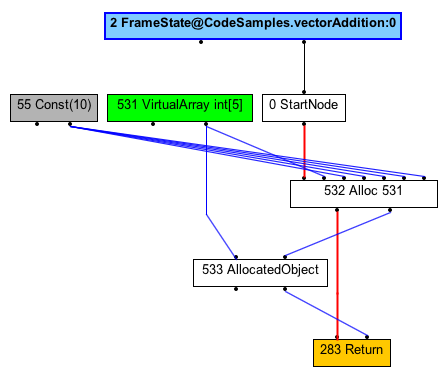
\includegraphics[width=0.7\textwidth]{graphics/loop-inline.png}
	\caption{Graal HIR created for a vector addition using two array literals}
	\label{fig:vector-inline}
\end{figure}

The format for graph visualisations is the following:
\begin{itemize}
	\item Red edges represent control flow
	\item Blue edges represent memory dependence
	\item Black edges are defined as edges which are not control flow or memory dependence. In reality, they are mainly used for associating \texttt{FrameState} nodes where appropriate
\end{itemize}

The text inside nodes uses the following format:

\texttt{<node-id> NodeName <additional>}

In some cases, \texttt{<additional>} contains the value associated with the code (for subtypes of \texttt{ValueNode}). Node IDs are unrelated to the ordering within the graph. Time is represented on the y-axis of the graph, flowing down the page.

\autoref{fig:vector-inline} is a representation of a vector addition using two \texttt{int} array literals as arguments. The original source code contains a loop, which itself contains two array load operations, an addition and an array store operation. From it, we can see clearly the different kinds of node relationships in Graal's IR. The \texttt{StartNode} is the start of the method, which is followed by an allocation (notice that the loop was been optimized away by Graal), the result of which is then returned from the method.

The allocate has two actual memory dependencies:

\begin{itemize}
	\item A \texttt{VirtualArray} node is used to create an array. We can see that the type of this array is \texttt{int[]} with length five.
	
	\item A \texttt{ConstantNode} is referenced five times, one for each position of the array.
\end{itemize}

Without both of these dependencies, the compiler cannot create the array, and assign the correct values. Note that, because the JVM allocates default values of zero to declared-yet-unassigned variables, if the \texttt{ConstantNode} was not used, the array would consist of zeros.

\section{Graph Transformations} \label{sec:graal/transformations}
One of the ways the abilities of Graal are manifested is through it's capacity to apply transformations to the various intermediate representations. The main use for this is to allow users of the compiler to add custom behaviour at the various stages of the compilation process, but the mechanism extends to additional uses. For example, custom behaviour can be inserted into programs, as well as the graphs dumped for inspection in external tools\footnote{One such tool is the `Ideal Graph Visualiser', which is included in the Graal repository.}.

As of the time of writing, Graal uses a hybrid approach to transforming graphs between the IRs - suites and phases. They are, in effect, essentially the same thing - they both consist of a sequence of transformations (in Graal terminology, a \textit{phase}) which are applied to a graph in a well-defined order (although the user can change the ordering if required, as well as disable certain phases via \texttt{com.oracle.graal.phases.PhasePlan.disablePhase()}. The result of a sequence of phases is the representation used at the next lower-level of abstraction. The three phases in Graal are high-level, mid-level, and low-level.

\small{\textit{Todo: clear up the difference between runtime-specific lowering and target-specific lowering.}}

The high-level phase is used mainly for the graph-building phase. Graal uses the concept of \texttt{ResolvedJavaMethod}s, which are internal `linkages' to constant pools found within \texttt{.class} files. It is also used for runtime-specific lowering\footnote{\emph{Lowering} is a mechanism to convert a complex bytecode into a simpler one, much like the difference between RISC and CISC architectures}, for example to handle multiple machine instruction set architectures - although the Java language is unconcerned with JVM implementation details such as the endianness of the machine's CPU, the runtime must, by definition, be aware of this fact. Examples of runtime-specific lowering are found throughout Graal, but examples include multiple implementations of the \texttt{GraalRuntime} interface - one for each ISA that Graal supports. Single Static Assignment (SSA) form is used at the high-level in order to allow for optimisations to be performed.

Mid-level phases remove the SSA form, and includes target-specific lowering. The low-level phases are analogous to the backends of more traditional compilers, and deals with low-level issues such as register allocation and code generation.

	\subsection{The \texttt{.class} File Format - Constant Pools}
	In order to properly understand \texttt{ResolvedJavaMethod}s, one needs to understand some parts of the \texttt{.class} file format. The source for this section is the Java Virtual Machine specification \citep[p.~69]{JVMSpec}.
		
	\texttt{.class} files are structured containers for Java bytecode streams. However, they are not `plain old data structures', as would be indicated by that description. Instead, they are laid out in such a way to increase performance for the JVM.
				
	Unlike some other executable file formats, the JVM does not rely on the (relative) positions of the various kinds of definition permitted. In this context, constants refer to \emph{all} immutable identifiers - and not simply to the language-level construct of constants (\eg, \texttt{public static final int THOMAS\_KLAUS = 9;}). Each constant has an entry in the \emph{constant pool} - a table containing \texttt{cp\_info} structures. A \texttt{ResolvedJavaMethod} contains a link to the offset of a \texttt{cp\_info} structure for a method.
	\chapter{Dynamic Instrumentation} \label{chp:instrumentation}
\section{Introduction} \label{sec:instrumentation/introduction}
There are two main approaches to dynamic instrumentation: automatic, and manual. We consider both of them, using Graal for an automatic, dynamic approach. We conclude by showing that, currently, it is not yet possible to use Graal for automatic instrumentation -- the reason for this is explained. As an alternative, manual instrumentation is used, and we explain the disadvantages and impact of this approach.

\section{Automatic Approaches - Graal} \label{sec:instrumentation/automatic}
	In this context, an automatic approach to instrumentation is a technique that can be applied directly at compile-time (or just before run-time in an agent-like fashion). Such approaches require no human intervention whatsoever, and have the additional advantage of having access to additional compile-time meta-data which is not possible to gain at run-time or using manual instrumentation.

	An automatic approach based on Graal was investigated. Graal was chosen because it is the most flexible approach: it allows the combination of compile-time evaluation, as well as run-time evaluation of the dependency algorithms.
	
	As mentioned, Graal uses various different forms of intermediate representation, based on graphs (see section \ref{sec:graal/ir}). In principle, it should be possible to modify these graphs in order to invoke the instrumentation (described in chapter \ref{chp:runtime}).
	
	Modifying graphs in Graal is made easy through a simple API. A user can define custom phases (see section \ref{sec:graal/transformations}). Pseudocode for this is as follows:
	
	\begin{lstlisting}[caption=Sample code for adding a phase and manipulating a graph,label=list:graph-trans]
	// create the phase
	public class MyPhase extends Phase {
	    @Override
	    protected void run(StructuredGraph graph) {
	        // modify the graph
	        for (LoadIndexedNode node:
	            graph.getNodes(LoadIndexedNode.class)) {
	            graph.addAfterFixed(node,
	                graph.add(new MyCustomNode()));
	        }
	    }
	}
	
	// add the phase
	Suites s = Graal.getRequiredCapability(SuitesProvider.class)
	    .createSuites();
	s.getHighTier().appendPhase(new MyPhase());
	\end{lstlisting}
	
	The call to \texttt{getHighTier()} can be replaced with equivalent methods for the other IRs (\ie, \texttt{getLowTier()} and \texttt{getMidTier()}.
	
	As we can see in figure \ref{fig:access-index}, which displays the high-level graph for a simple method that takes an array actual parameter and returns index $0$ of that array, there are specialised nodes for array accesses: \texttt{LoadIndexedNode}. Note that there is also an equivalent for array store operations, \texttt{StoreIndexedNode}.
	
	\begin{figure}[h]
		\centering
		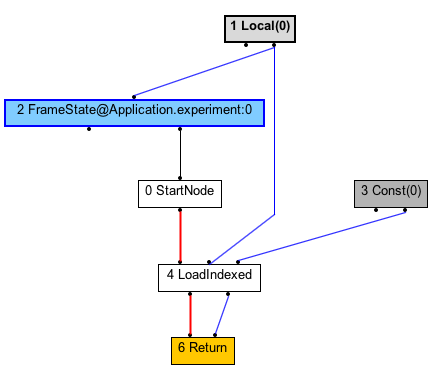
\includegraphics[width=.7\textwidth]{graphics/access-index.png}
		\caption{A high-level graph (with inlining disabled) for a simple method taking an array actual parameter, returning index 0}
		\label{fig:access-index}
	\end{figure}
	
	This is the basis for selecting the appropriate nodes to instrument. One additional advantage of Graal is the richness of the information available at compile-time. Figure \ref{fig:graal-meta} shows all the available information, as seen in Eclipse's debugger.
	
	\begin{figure}[h]
		\centering
		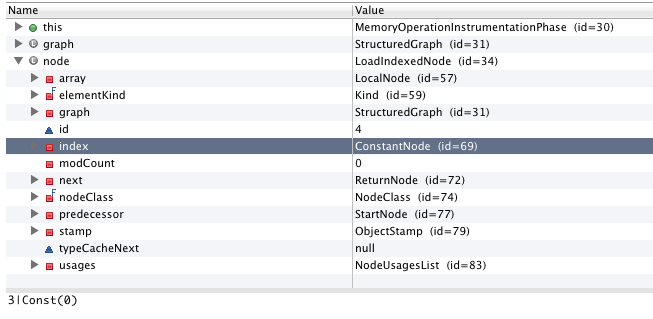
\includegraphics[width=0.8\textwidth]{graphics/graal-metadata.png}
		\caption{Information available at compile-time for the \texttt{LoadIndexedNode} shown in figure \ref{fig:access-index}}
		\label{fig:graal-meta}
	\end{figure}
	
	The availability of predecessor and next nodes, as well as nodes representing indexes (in this case, a \texttt{ConstantNode}) highlights another advantage of using Graal for these transformations - static analysis is possible, which means that instrumentation can be disabled if dependencies can be proven statically. 
	
	There are several possibilities for adding instrumentation in Graal.
	
	\begin{enumerate}
		\item \label{item:instr1} Add a custom node type, which is lowered to an invoke instruction after each applicable node.
	
		\item \label{item:instr2} Replace the nodes in question with a custom node that implements the same operation in addition to the required behaviour.
	
		\item \label{item:instr3} Javassist includes a method for replacing all array accesses with method calls \citep{JavassistDocs}. It may be possible to use Graal to replace the method call targets where instrumentation is required. In cases where no instrumentation is required, the method would return the array value (or perform the store), which would then be inlined by the compiler.
	\end{enumerate}
	
	In cases \ref{item:instr1} and \ref{item:instr2}, then node would need to implement \texttt{Lowerable}, an interface in Graal that allows nodes to be lowered between IR levels.
	
	\textit{However}, there is currently a limitation in Graal which means that it is not currently possible to insert calls to (static) methods. This is because there is no \emph{bytecode index} (or BCI) for the interpreter to return to if a deoptimisation occurs (details on Graal's deoptimisation mechanisms are available in section \ref{sec:graal/deopt}). Since methods calls cannot be guaranteed to be deoptimisation-free, they cannot be inserted into graphs. Any static methods that modify abstract data types (\ie, the storage formats described in section \ref{sec:runtime/storage}) cannot be assumed to be deoptimisation free. Modifying a data structure violates the optimisation assumptions, causing a deoptimisation. The interpreter then tries to resume from the BCI of the invoke. However, there is no BCI associated with inserted invocation, meaning that the interpreter cannot resume in the event of the inevitable deoptimisation. The end result is that insertation of arbitrary behaviour through invoke nodes to static methods is not currently possible in the Graal system.
	
	To illustrate the concept of BCIs, consider the following example. In Java bytecode, each instruction has an associated index (this example was compiled using \texttt{javap -c} from a basic `hello, world!' application):
	
	\begin{verbatim}
	Compiled from "Hello.java"
	public class Hello {
	  public Hello();
	    Code:
	       0: aload_0       
	       1: invokespecial #1    // Method java/lang/Object."<init>":()V
	       4: return        
	
	  public static void main(java.lang.String[]);
	    Code:
	       0: getstatic     #2    // Field java/lang/System.out:Ljava/io/PrintStream;
	       3: ldc           #3    // String Hello, world
	       5: invokevirtual #4    // Method java/io/PrintStream.println:
	       (Ljava/lang/String;)V
	       8: return        
	}
	
	\end{verbatim}
	
	We can clearly see the BCIs of the various operations: the \texttt{invokespecial \#1} has a BCI of 1, and so on.

	This is a limitation of the Graal platform. In the coming months, the Graal core developers are adding this required feature. Once the feature has been added, it is a simple modification (as the infrastructure has already been created) to add this into Graal. Indeed, the required infrastructure for this transformation has been created -- once the support for it is available, only would need to enable the transformations.
	
	As an alternative, we used manual instrumentation (section \ref{sec:instrumentation/manual}). Although this does have the disadvantage of requiring both source-code access as well as human effort, this will not affect the results or correctness of the evaluation as the semantics are equivalent. The results and conclusions of this report will not be affected by this shortcoming of Graal. The required framework and infrastructure has already been developed, the mechanism through which the framework is used cannot affect the results in this case.
	
\section{Manual Approaches} \label{sec:instrumentation/manual}
The major alternative to automatic instrumentation is manual instrumentation, where the user manually performs the required transformations in the source code.

These transformations consist of replacing array access and store operations with method calls, whilst adding relevant metadata if required. For example, consider the following array access:

\begin{lstlisting}[label=list:array-access,caption=Standard array access in Java]
int c = a[b];\end{lstlisting}

Manual instrumentation refers to replacing this operation, and all such operations, with the following (or equivalent):

\begin{lstlisting}[label=list:instrumented-array-access,caption=Instrumented array access]
int c = access-array(a, b);\end{lstlisting}

The \texttt{array-access} method (and the implied \texttt{array-store} method) performs the dependency checking algorithms using the techniques as described in section \ref{sec:runtime/analysis/online}.
	
\section{Summary} \label{sec:instrumentation/summary}
In this section, we have considered the use of Graal for automatic instrumentation. We have seen that, due to a limitation in the current version of Graal, it is not possible to add arbitrary static method invoke instructions. Regardless of this limitation, there are other possible approaches that could also (in principle) be used for automatic instrumentation.

Lastly, we have seen how manual instrumentation is possible, and the reasons why the alternative approach used (manual instrumentation) will not affect the results or conclusions of this dissertation.
	\chapter{The Runtime Library} \label{chp:runtime}
\section{Introduction} \label{sec:runtime/introduction}
In this chapter, the work performed towards implementing the runtime library, known as Locomotion, is presented. This library handles several core functions critical to the infrastructure of the application:

\begin{itemize}
	\item Functions for collecting trace analyses
	\item Implementations of trace storage backends
	\item Algorithms for offline and online dependency analysis
\end{itemize}

The programs described within this chapter are open-source, released under The University of Edinburgh GPL license. They are available at \url{https://github.com/chrisatkin/locomotion}.

The fully-qualified package identifier for the runtime library is\\\texttt{uk.ac.ed.inf.icsa.locomotion.instrumentation}.

\section{Trace Storage} \label{sec:runtime/storage}
Generating traces for large programs -- the kind of programs which would benefit from hot-loop analysis -- requires a large amount of storage as it scales linearly with the number of memory operations ($S=O(n)$). Although the number of storage operations conforming to the requirements in a program may be relatively small, this number is increased when the standard library is included.

The main problem that the storage format must be able to determine is this. Given trace $T$ and access $\alpha$, is $\alpha \in T$?
	
	\subsection{Exact Approaches: Hash Tables and Sets} \label{sec:runtime/storage/exact}
	Exact approaches provide an accurate deterministic response to this question. They are not probabilistic or statistical in nature.

	A hash function maps keys to indexes, where buckets are stored. Buckets contain all items with the same key. Ideally, a lookup of $T=O(1)$ is possible (\ie, a hash function with ideal distribution). Worst-case cost is $T=O(n)$, in the case of multiple collisions or a low load factor, as the bucket will need to be traversed sequentially to find the item.
		
	It is common to use hashing by division for the hash function:
		
	\[
		f(k) = k \bmod{D}
	\]
		
	Where $k$ is the key and $D$ is the size (\ie, number of positions of the hash table) \citep{DSandAlgsCpp}.
		
	The constant-time lookup assumes that the \textit{load factor} $L$ is bounded below some constant. The load factor is computed by $L=\frac{n}{k}$.
		
	Figure \ref{fig:hash-table} demonstrates a simple hash table without collisions.
		
	\begin{figure}
		\centering
		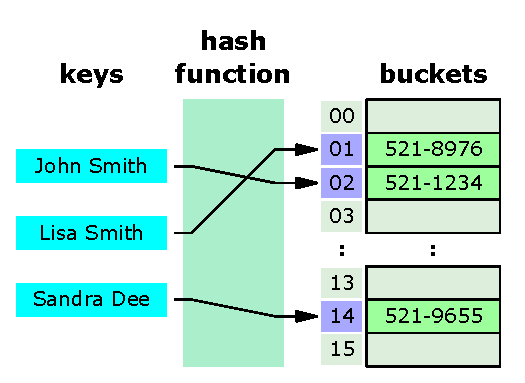
\includegraphics[width=0.7\textwidth]{graphics/hash-table.pdf}
		\caption{A simple hash table for a phone book \citep{HashTableWikiDiagram}}
		\label{fig:hash-table}
	\end{figure}

	\subsection{Probabilistic Approaches: Bloom Filters} \label{sec:runtime/storage/probabilistic}
	The main disadvantage to using exact approaches is that the storage required scales linearly such that $S=O(n)$. For anything but the most trivial programs, this means that it becomes infeasible to store traces for all memory operations.
	
	One alternative is the use of Bloom Filters \citep{Bloom1970}. A Bloom Filter is a randomised data structure which supports membership queries, with the possibility of false positives. In the context of parallelism detection, this means that we may conclude that a loop is not parallelisable when in reality, it is.
		
	The operation of a Bloom Filter is simple: there exists a bit vector of size $m$ and a number $k$ of hash functions (which could use universal hashing \citep{Carter1979}). Upon insertation of an item $i$, for each hash $k_n$ the value of $v_n=k_n(i)$ is computed, which is an integer in the range $0..m$. The corresponding index of the vector is then set to $1$.
		
	\begin{figure}[h!]
			\centering
			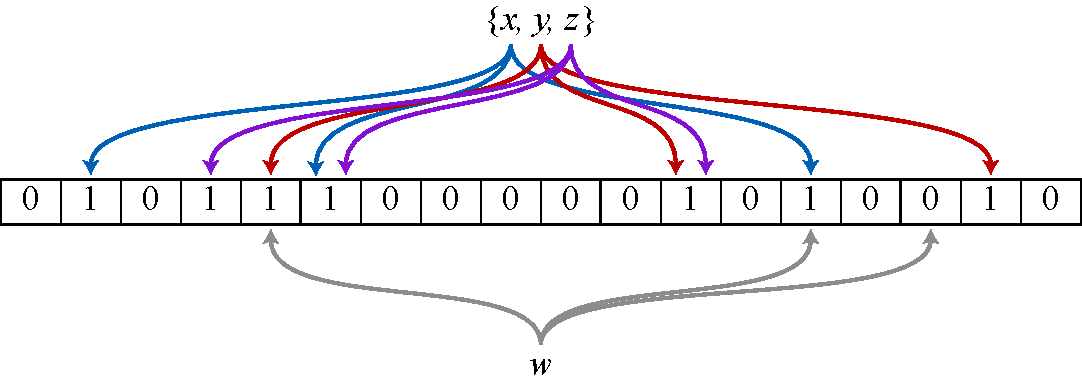
\includegraphics[width=0.8\textwidth]{graphics/bloomfilter.pdf}
			\caption{Bloom filter operation with $m=18$ and $k=3$ \citep{BloomFilterWikiDiagram}}
			\label{fig:bloom-filter}
	\end{figure}
		
	To test membership for an item, feed the item to each hash function. If all the corresponding indexes are $1$, then the item \emph{may} be contained within the filter - if any of them are $0$, then the item is definitely not.
	
	For a given number of entries $s$ and a bit vector of size $m$, we need to use $k$ hash functions such that:
	
	\begin{equation}
		k = \frac{m}{s} \ln 2
		\label{eqn:optimal-hashes}
	\end{equation}
	
	The error rate is defined as:
	
	\[
	\sigma = 0.5^k
	\]
	
	In essence, the longer the bit vector, the more accurate the filter becomes - at the expense of increasing space requirements. If $m=\infty$, then there are no false positives - the filter becomes accurate and deterministic (for a fixed set of $k$).
	
	\citet{Swamidass2007} show is that the number of elements within a Bloom Filter can be estimated by:
	
	\[
	E = -n \ln \frac{1-n/n}{k}
	\]
	
	% return (long) (-n * Math.log(p) / (Math.log(2) * Math.log(2)));
	
	It is possible to calculate the theoretical optimal length of the bit vector $m$ from the number of expected insertions $n$ and the \textit{false positive rate} $p$. This is defined as

	\begin{equation} \label{eqn:optimal-bits}
		m = -n \times \log(p) \div \left( \log(2) \times \log(2) \right)
	\end{equation}
	
	It is possible to use equation \ref{eqn:optimal-bits} to compute the memory usage for given $m$ and $p$, this is shown in figure \ref{fig:opt-bits}.
	
	\begin{figure}
		\begin{gnuplot}[terminal=pdf]
			set ylabel 'bit vector length'
			set xlabel 'expected insertions'
			set xr [1:10000000]
			set grid
			
			# Line style for grid
			set style line 81 lt 0  # dashed
			set style line 81 lt rgb "#808080"  # grey
			
			set xtics nomirror
			set ytics nomirror
			
			set key top left
			
			f(n, p) = -n * log(p) / (log(2) / log(2))
			
			plot f(x, 0.3) title 'p = 0.3' lw 3,\
				 f(x, 0.03) title 'p = 0.03' lw 3,\
				 f(x, 0.003) title 'p = 0.003' lw 3,\
				 f(x, 0.0003) title 'p = 0.0003' lw 3
		\end{gnuplot}
		\caption{Plot showing bit vector length versus expected insertations for various false probability rates}
		\label{fig:opt-bits}
	\end{figure}
	
	The main advantage of bloom filters is that the space complexity is constant $S=O(c)$, where $c$ is the size of the bit vector. This will allow memory overhead to be substantially lower, whilst still retaining $T=O(1)$ lookup time complexity. As mentioned above, this is a significant (factor $n$) improvement over the exact approach.

	However, lookup time in bloom filters is asymptotically greater than the hash-based alternative. Unlike the hashing-based approach which has, with an optimal load factor, a lookup time of $T_{lookup}^{hash}=O(1)$, a bloom filter has a lookup time of $T_{lookup}^{bloom}=O(k)$ (where $k$ is the number of hash functions). This is unlike amongst array/vector-based approaches, which in many cases are $T=O(1)$. As the number of optimal hash functions is dependent on the number of expected entries and the bit vector size (see equation \ref{eqn:optimal-hashes}), it is predicted that execution time will increase slightly as a result, with the assumption that the hashing-based approach is operating efficiently (\ie, with an adequate load factor).
	
	\subsubsection{Implementations} \label{sec:runtime/storage/probabilistic/impls}
	Unlike hash sets, where a canonical implementation exists in the form of \texttt{HashSet} within the Java API, there is not a single canonical implementation of bloom filters for Java. Naturally, however, there are many third-party implementations, each of which have different properties. Although where appropriate, these properties will still conform to the theoretical time and space complexities presented above, asymptotic performance is only one aspect of `real-world' performance.
	
	The first implementation that exists is from the Google Guava project, which is a collection of APIs that applications commonly require. The Google implementation is a general-purpose bloom filter implementation, based around the concept of `Funnels'. Funnels stream primitive values into \texttt{PrimitiveSinks}, of which a bloom filter is an example. In this way, a Funnel is a kind-of interface to the bloom filter, allowing the user to specify only certain values which should be considered for hashing. Additionally, they permit high performance as string-based representations, another `general-purpose' representation, require additional overhead.
	
	The alternative implementation used is taken from the Apache Cassandra project. Cassandra is a distributed, highly-scalable database management system, and it uses bloom filters to improve performance on disk lookup \citep{CassandraArch}. Although this implementation is not considered a standalone implementation in the same way the Google Guava implementation is, it is still easy to remove from Cassandra.
	
	The key difference that this implementation is the difference in hash function. Instead of a custom function used in Guava (which is based around \citet{Swamidass2007}), Cassandra instead uses the MurmurHash function \citep{MurmurHash}. MurmurHash is known to be a high-performance, general-purpose hashing mechanism, and may prove superior to the custom methodology use in Guava. The reason that MurmurHash has higher performance is because it operates on 4 bytes per operation, rather than the single byte used in many other hash functions. However, this implementation is optimised towards strings, requiring all objects to be converted to string representation before hashing. This may be a source of overhead.
	
	In chapter \ref{chp:results}, we will begin with a comparison between these bloom filter algorithms, continuing with the rest of the analysis with the implementation with the highest performance.

\section{Dependency Analysis Algorithms} \label{sec:runtime/analysis}
	Computing dependency between two operations is of critical importance to this project; an efficient algorithm is important.
	
	\subsection{Why are dependencies important?} \label{runtime/analysis/why}
	Dependencies, also called \textit{hazards} (especially in processor architecture literature) are of critical importance to automatic parallelisation as they determine whether (or not) a loop can be automatically parallelised. If there is a dependence, the statements cannot be executed in parallel without additional transformation (which may be intractable) of the program\footnote{One example of where such a transformation is possible is a summation of a counter: \texttt{for int i = 0 to n: i++}. This program can be broken down into a tree of tasks and executed in a divide-and-conquer fashion, which is easily parallelisable}. However, such transformations are likely not possible for compilers to perform automatically. 
	
	\subsection{Dependency Theory} \label{sec:runtime/analysis/theory}
	From \citet[p.~37]{Allen2000}, there is a data dependence from statement $\sigma_x$ to statement $\sigma_y$ (where $T(\sigma_x) \rightarrow T(\sigma_y)$\footnote{For two statements $x$ and $y$, $x \rightarrow y$ iff there is a viable execution path between $x$ and $y$}) if and only if:
	
	\begin{enumerate}
		\item both statements access the same memory location and at least one of them stores into it
		\item there is a feasible run-time execution path from $\sigma_x$ to $\sigma_y$
	\end{enumerate}
	
	There are several kinds of inter-iteration dependency \citep[p.~526]{Ibbett2009,ArchitectureBook}. In this section, $R(\alpha_x)$ denotes the set of addresses/locations read by access $\alpha_x$, and $W(\sigma_x)$ denotes the set of addresses read by access $\sigma_y$.
	
	\begin{itemize}\label{fig:dep-kinds}
		\item \textbf{Write-after-write} or \textit{output dependency}: given two statements $\sigma_x$ and $\sigma_y$, there is a write-after-write dependency if a total ordering is required for $\sigma_x$ and $\sigma_y$. For example:
		
		\begin{verbatim}
		R3 = R1 + R2
		R3 = R3 + R4
		\end{verbatim}
		
		If the second statement were executed before the first statement, program correctness would be violated, so speculative execution is not possible.
		
		Formally, there is an output dependence iff $W(\sigma_x) \cap W(\sigma_y) \neq \varnothing$.
		
		Output dependence for two statements $\sigma_x$ and $\sigma_y$ is denoted as $\sigma_x \delta^0 \sigma_y$.
		
		\item \textbf{Write-after-read} or \textit{antidependency}: given two statements $\sigma_x$ and $\sigma_y$, there is a write-after-read dependency if evaluation of $\sigma_y$ is dependent on the evaluation of $\sigma_x$:
		
		\begin{verbatim}
		R1 = R2 + R3
		R2 = R4 + R5
		\end{verbatim}
		
		In this case, if the statements are re-ordered, the wrong value of \texttt{R2} will be used.
		
		There is an antidependency iff $R(\sigma_x) \cap W(\sigma_y) \neq \varnothing$.
		
		Antidependence for two statements $\sigma_x$ and $\sigma_y$ is denoted as $\sigma_x \delta^{-1} \sigma_y$.
		
		\item \textbf{Read-after-write} or \textit{true dependency}: given two statements $\sigma_x$ and $\sigma_y$, there is a read-after-write dependency if $\sigma_y$ stores the value (or derivative value) of $\sigma_x$:
		
		\begin{verbatim}
		R1 = R2 + R3
		R4 = R1 + R5
		\end{verbatim}
		
		If the statements are reordered, either a stale value of R1 will be used, or R1 may not have been initialized.
		
		There is a true dependency iff $W(\sigma_x) \cap R(\sigma_y) \neq \varnothing$.
		
		True dependency for two statements $\sigma_x$ and $\sigma_y$ is denoted as $\sigma_x \delta \sigma_y$.
	\end{itemize}
	
	Combining these, we gain the \textbf{Bernstein Condition}. There is a dependence between $\sigma_x$ and $\sigma_y$ iff:
	
	\begin{equation} \label{eqn:bernstein}
	\left[ R(\sigma_x) \cap W(\sigma_y) \right] \cup \left[ W(\sigma_x) \cap R(\sigma_y) \right] \cup
	\left[ W(\sigma_x) \cap W(\sigma_y) \right] \neq \varnothing
	\end{equation}
	
	There is also a theoretical dependency that can be detected by the framework, read-after-read, but since this does not cause two iterations to be dependent, they are not considered by the framework.
	
	For an arbitrary loop in which the loop index $I$ runs from $L$ to $U$ in steps of $S$, the iteration number $i$ of a specific iteration is equal to the value $\frac{I-L+S}{S}$, were $I$ is the value of the index on that iteration.
	
	Given a nest of $n$ loops, the \textit{iteration vector} $i$ of a particular iteration of the inner-most loop is a vector of integers that contain the iteration numbers for each of the loops in order of nesting level. $i$ is given by $i=\{i_1, i_2, ..., i_n\}$ where $ik$, $1 \leq k \leq n$, represents the iteration number for the loop at level $k$.
	
	There exists a loop dependence from statement $\sigma_1$ to $\sigma_2$ in a common next of loops iff there exists two iteration vectors $i$ and $j$ for the nets, such that:
	
	\begin{enumerate}
		\item $i < j \lor i = j$ and there is an execution path from $\sigma_x$ to $\sigma_y$ in the body of the loop
		\item Statement $\sigma_x$ accesses memory location $m$ on iteration $i$ (access $\alpha_x$) and statement $\sigma_y$ accesses location $m$ on iteration $j$ (access $\alpha_y$)
		\item Either $\alpha_x$ or $\alpha_y$ is a store
	\end{enumerate}
	
	Thus, the following problem declaration can be constructed for computing dependencies:
	
	Let $i^l_n$ be the set of memory accesses for iteration $n$ in loop $l$. For a memory access $\alpha \in i^l_n$, determine whether there exists a previous iteration such that $\alpha \in i^l_{n-c}$ for some integer $c$. Additionally, for an access $\alpha_i$ and previous access $\alpha_{i-c}$, $kind(\alpha_i) \neq read \land kind(\alpha_{i-c}) \neq read$.
	
	In addition, there are two kinds of loop dependence.
	
	\begin{itemize}
		\item \textbf{Loop-carried dependence}: $\sigma_x$ can reference a common location $m_c$ on an iteration, $\sigma_y$ can reference the same location $m_c$
		\item \textbf{Loop-independent dependence}: $\sigma_x$ and $\sigma_y$ can both access $m_c$ on the same iteration, but with $\sigma_x$ preceding $\sigma_y$ during execution
	\end{itemize}

	\subsection{Offline Algorithms} \label{sec:runtime/analysis/offline}
	An offline algorithm means that any processing is performed after the trace has been collected \citep[p.~525-526]{TAOCPvol2}. It is the simplest form of dependency analysis algorithm, but it show poor performance. For a number of loops $l$ with an average of $i$ iterations each, where each iteration has an average of $o$ operations, then $T_{offline}=O(lio)$.
	
	\begin{algorithm}
		\caption{Offline dependency algorithm}
		\label{alg:offline-dependency}
		\begin{algorithmic}[1]
			\STATE $d \gets \varnothing$ %\COMMENT{$d$ is the set of dependencies}
			\FORALL{loops $l$}
				\STATE $p \gets \varnothing$ %\COMMENT{$p$ is the set of previous iterations}
				\FORALL{iteration $i \in l$}
					\FORALL{access $\alpha \in i$}
						\FORALL{$p_{\alpha} \in p$}
							\IF{$\alpha \in p{_\alpha}$}
								\STATE $d \gets \alpha$
							\ENDIF
							
							\STATE $p \gets \alpha$
						\ENDFOR
					\ENDFOR
				\ENDFOR
			\ENDFOR
		\end{algorithmic}
	\end{algorithm}
	
	This offline algorithm has several disadvantages. Not only is its runtime particularly poor (we can achieve at least a factor $l$ speed-up using an online algorithm), but because it requires a complete trace of accesses per iteration, it is unsuitable for  detecting dependencies at run-time. Algorithm \ref{alg:offline-dependency} outlines the offline algorithm.

	\subsection{Online Algorithns} \label{sec:runtime/analysis/online}
	\begin{figure}
			\centering
			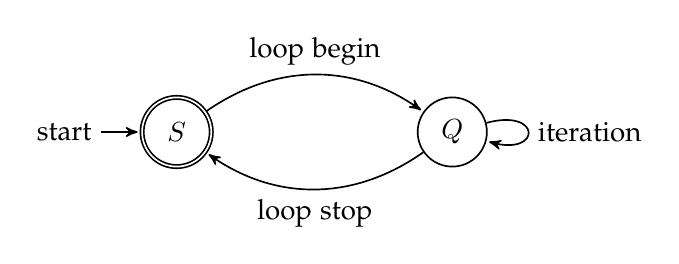
\begin{tikzpicture}[->,>=stealth',shorten >=1pt,auto,node distance=3.5cm,semithick, bend angle=35]
				\node[initial,accepting,state]	(q1)					{$S$};
				\node[state]					(q2)	[right of=q1]	{$Q$};
				
				\path[->]
					(q1)	edge [bend left ] node {loop begin} (q2)
					(q2)	edge [bend left] node {loop stop} (q1)
							edge [loop right] node {iteration} (q2);
					
			\end{tikzpicture}
			\caption{Finite state machine for the online algorithm}
			\label{fig:online-fsm}
		\end{figure}
		
	An online algorithm for this problem is one that runs with a sequential input of values. An online algorithm is superior because it shows better performance characteristics asymptotically, $T_{online} = O(io)$, and it runs in conjunction with the program. This allows Locomotion, in theory, to advice any JIT compilers of optimisations to perform. Figure \ref{fig:online-fsm} represents the finite state machine for the algorithm.
	
	\begin{algorithm}
		\caption{Online dependency algorithm}
		\label{alg:online-dependency}
		\begin{algorithmic}
			\STATE $d \gets \varnothing$ %\COMMENT{$d$ is the set of dependencies}
						\FORALL{loops $l$}
							\STATE $p \gets \varnothing$ %\COMMENT{$p$ is the set of previous iterations}
							\FORALL{iteration $i \in l$}
								\FORALL{access $\alpha \in i$}
									\FORALL{$p_{\alpha} \in p$}
										\IF{$\alpha \in p{_\alpha}$}
											\STATE $d \gets \alpha$
										\ENDIF
										
										\STATE $p \gets \alpha$
									\ENDFOR
								\ENDFOR
							\ENDFOR
						\ENDFOR
		\end{algorithmic}
	\end{algorithm}

\section{Implementation Details} \label{sec:runtime/implementation}
In this section, we consider the techniques used to implement the runtime library and online dependency algorithm from a software engineering perspective.

	\subsection{Entry Point} \label{sec:runtime/implementation/entry-point}
	The main entry point to the instrumentation is the \texttt{InstrumentSupport} class. It includes an \texttt{Instrument}, which is an implementation of instrumentation. There is also a number of static methods for accessing the instrumentation framework, such as starting and ending timers (and getting time differences in nanoseconds) and flushing the instrument buffers. Figure \ref{fig:instrument-support} shows the class diagram with public methods for \texttt{InstrumentSupport}.
	
	\begin{figure}
		\centering
		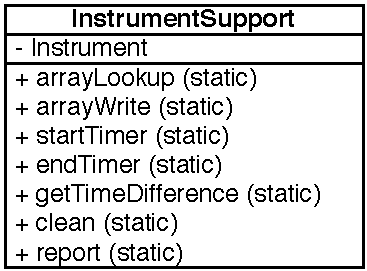
\includegraphics[width=0.4\textwidth]{graphics/instrument-support.pdf}
		\caption{Class diagram for \texttt{InstrumentSupport}}
		\label{fig:instrument-support}
	\end{figure}
	
	\subsection{Instrument Implementation} \label{sec:runtime/implementation/instrument}
	\texttt{InstrumentSupport} is initalised at load-time with an \texttt{Instrument} (via static blocks). \texttt{Instrument} is an implementation of instrumentation, and it has a configuration. This configuration contains parameters such as whether the instrumentation should be enabled and so on.
	
	The user-facing methods for trace collection have the following signatures:
	
	\begin{lstlisting}[caption=Method signatures for instrumentation methods,label=lst:sigs]
	public static <T> void
	arrayLookup(T[] array, int index, int i, int id);
	
	public static <T> void
	arrayStore(T[] array, int index, T value, int i, int id);\end{lstlisting}
	
	The arguments are:
	
	\begin{itemize} \label{items:trace-args}
		\item \texttt{T[] array}: the array upon which the operation is occuring
		\item \texttt{int index}: the array index in question
		\item \texttt{int i}: the value of the iteration variable
		\item \texttt{T value}: the value being written to the array at the index
		\item \texttt{int id}: a unique loop identifier
	\end{itemize}
	
	The Java generics system was leveraged in order to reduce the amount of code required to implement the collection; it is important to recognise that the Java type system allows the trace collection mechanism to be unconcerned with the type of the array being accessed (and the type of the item being inserted if appropriate).
	
	Although it would be possible to use the above generics-based methods for all data types, this would require the use of the object-oriented wrapper libraries (also called the reference types) for \texttt{int} $\rightarrow$ \texttt{Integer}, \texttt{float} $\rightarrow$ \texttt{Float} and so on. This would have the disadvantage of incurring the overhead of autoboxing \citep{boxing} in the library.
	
		\subsubsection{Java Auto(un)boxing} \label{sec:runtime/implementation/instrument/boxing}
		Despite being an object-oriented language, Java has several non-object-oriented types. These are known as \textit{primitive values}. They are not part of the standard object-hierarchy, and no methods can be called upon them. The primitive types are \texttt{int}, \texttt{long}, \texttt{char}, \texttt{float}, \texttt{double}, \texttt{boolean} and \texttt{short}.
		
		Each primitive type has a corresponding reference type (named as such because Java uses pass-by-reference for objects), which is an object and hence part of the class hierarchy.
		
		Although this approach does have some advantages -- primitive types require less over head than the object-oriented value types -- there are some disadvantages -- namely, enable interoperability between the two.
		
		This process is called auto boxing (in the case of primitive-to-reference type occurs) or auto unboxing (where reference-to-primitive type occurs). The advantage of this approach is that it simplifies programming and reduces `crufty' code. For example, adding two \texttt{Integer}, \texttt{a} and \texttt{b} doesn't require \texttt{Integer c = a.add(b);}, but instead the more natural \texttt{Integer c = a + b} can be used. In this case, \texttt{a} and \texttt{b} will be auto-unboxed to primitive types, the addition is performed and the result is autoboxed back to \texttt{Integer}.
		
		However, this automatic casting operation does occur a slight performance overhead, both in terms of memory and execution time. Although in most cases the overheads are small, for benchmarking a runtime system with somewhat significant overheads, another solution was opted for. Instead of only supporting value types, we \emph{also} support primitive types by overloading the appropriate methods. 
		
		In order to overcome this performance problem, the instrumentation has been optimised to consider both primitive types and reference types.
	
	\subsection{Trace Storage and Configuration} \label{sec:runtime/implementation/trace}
	The instrumentation includes implementations of both exact and inexact approaches to trace storage.
	
	The \texttt{Access} class provides an abstraction for an access. An \texttt{Access} represents an array access with an associated kind, index, number (``\textit{this iteration represents the $n$th access this iteration''}).
	
		\subsubsection{Exact - Hash Set} \label{sec:runtime/implementation/trace/hashset}
		For the exact implementation, I chose to use the standard Java Collections Framework \texttt{HashSet} class. This is for several reasons, such as:
		
		\begin{itemize}
			\item \textbf{Performance}: array lookup in hash maps is $T=O(1)$, assuming an equal distribution of hash codes. For this reason, \texttt{Access} also overrides the standard \texttt{hashCode()} implementation, so that any two accesses are equivalent iff the array ID and indexes match.
			
			\item \textbf{Uniform interface}: any member of the Collections framework includes by-default various capabilities, such as being \texttt{Iterable}, meaning enhanced for-each loops can be used.
			
			\item \textbf{Standard implementation}: the built-in implementation has been tested for bugs, and is (mostly) bug-free. A custom implementation could not be subjected to this same rigorous testing.
		\end{itemize}
		
		\subsubsection{Inexact - Bloom Filters} \label{sec:runtime/implementation/trace/bloom}
			Rather than creating a custom implementation of Bloom filters, I used an existing implementation in the form of Google Guava \citep{GuavaBloomFilter}.\
		
		There is a parent abstract class, \texttt{Trace} which specifies several standard methods that all interfaces must define (\texttt{add()}, \texttt{contains()} and \texttt{size()}). All implementations of traces inherit from this superclass. Figure \ref{fig:trace-classes} shows this hierarchy in detail.
		
		\begin{figure}
			\centering
			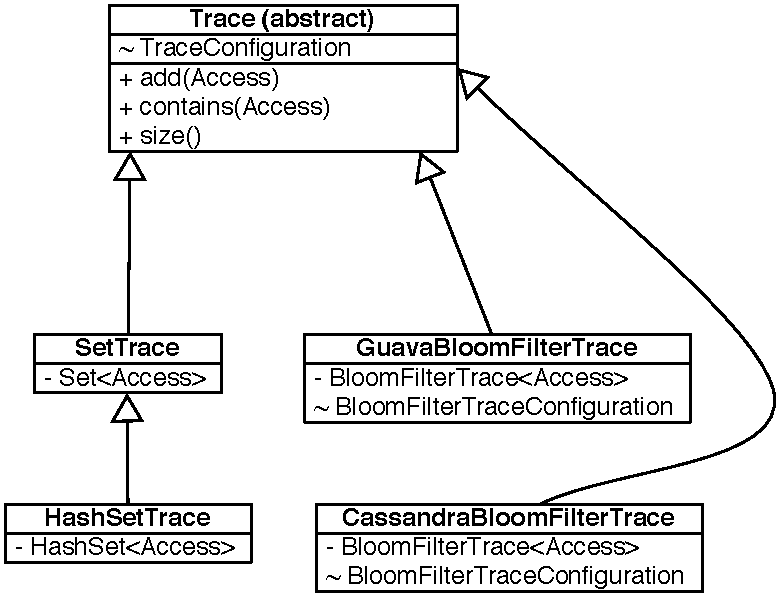
\includegraphics[width=0.7\textwidth]{graphics/trace-classes.pdf}
			\caption{Trace class hierarchy}
			\label{fig:trace-classes}
		\end{figure}
		
		A \texttt{TraceConfiguration} class is used to provide configuration details for the trace. There are no configuration variables used for hash sets, but for bloom filters this includes the initial size and the \texttt{Filter} used (an implementation detail as a result of the use of Google Guava). Dynamic configuration was preferred to constants as many experiments will need to be run, often with different variables.
		
		When a new access $\alpha$ in iteration $i$ and loop $l$ is detected, the library checks if $l$ is a new loop, or an existing one. If the loop is new, it instantiates a new \texttt{Loop} object, which holds the traces, as well as detecting whether an access is dependent. \texttt{Loop} stores two instantiations of the supplies \texttt{Trace} class - one for read and one for write operations. This is necessary in order to detect $\sigma_x \delta \sigma_y$, $\sigma_x \delta^0 \sigma_y$ and $\sigma_x \delta^{-1} \sigma_y$ dependencies, but not read-after-read dependencies. In order to use a single trace implementation, the semantics of the \texttt{hashCode()} and \texttt{equals()} methods, along with the \texttt{Comparable} access would need to be violated as a temporal dependence is introduced. Both bloom filters use \texttt{hashCode()} to determine an item is contained. It is not possible to use a $\sigma_x \delta \sigma_y$, $\sigma_x \delta^0 \sigma_y$ and $\sigma_x \delta^{-1} \sigma_y$ but not read-after-read dependencies.
		
		In order to detect dependencies, \texttt{Loop} checks all \emph{previous} iterations, using a $T=O(1)$ check on for containment within both read and write traces. Overall, for $n$ iterations the solution has a time complexity $T=O(n)$ and a space complexity $S=O(a)$, where $a$ is the number of accesses. Once a loop has been completed as detected by the finite state machine (see figure \ref{fig:online-fsm}), the accesses are deleted in order to reduce memory location.
		
		Dependencies are reported to the runtime via an exceptions mechanism. When a dependence is detected a special exception, \texttt{LoopDependencyException} is thrown, which is initialised with hazard metadata (which access is dependent, the kind of dependence, and the two iterations which the access occurs within). \texttt{LoopDependencyException} is a checked exception. The exception traverses up the stack until it reaches \texttt{Instrument}, which stores all exceptions of the same type in a linked list. This list is available to users of the framework, meaning full dependency information is available.

\section{Summary} \label{sec:runtime/summary}
In this chapter, the theory of dependence analysis has been introduced, as well as some practical approaches to implementing them. Both kinds of dependency checking algorithm (offline and online) have been covered, as well as implementation details of online algorithms in our framework.

Lastly, a software engineering-based approach to the design of the instrumentation framework was discussed.
	\chapter{Methodology} \label{chp:methodology}
\section{Introduction} \label{sec:methodology/introduction}

\section{Experimental Setup} \label{sec:methodology/setup}
The hardware used for the experiments is a mid-2009 MacBook Pro with the following specifications:
	
\begin{itemize}
	\item Intel Core 2 Duo P8800 @ 2.66GHz
	\item 8GB 1067MHz DDR3
	\item Nvidia GeForce 9600M GT 256MB
	\item Disks:
	\begin{itemize}
		\item Samsung SSD 830 Series 128GB via SATA-2
		\item Western Digital Scorpio Blue 1TB via SATA-2
	\end{itemize}
\end{itemize}

The software configuration is as follows:
\begin{itemize}
	\item OS X 10.8.4 (build 12E55)
	\item Java 7 update 25
\end{itemize}

All software used was the latest version available at the time of writing.

\section{Repeats} \label{sec:methodology/repeats}
In order to improve the results, each experiment was repeat three times. The average of the three repeats was used in plotting charts etc.

\section{Benchmarks} \label{sec:methodology/benchmarks}
	\subsection{Validation and Basic Testing} \label{sec:methodology/benchmarks/simple}
	The first `item of business' is to prove that the implementation of the instrumentation is correct. We ensure this by comparing the results of algorithms with pre-determined results to the output of the instrumentation.
	
	Since there are several kinds of dependency (see figure \ref{sec:runtime/analysis}), these benchmarks need to take this into account.
	
	\subsection{Parametric Benchmarks} \label{sec:methodology/benchmarks/parametric}
	In addition to basic verification, a parametric benchmark has been created. This benchmark -- called \textit{FractionalDependent} -- allows a user to specify 
	
	\subsection{Graph Processing Algorithms} \label{sec:methodology/benchmarks/graphs}
	
	\subsection{Java Grande} \label{sec:methodology/benchmarks/grande}
	Java Grande \citep{Smith2001,Bull2001} is a platform-independent benchmark for Java Virtual Machines and their associated compilers. Indeed, it is aimed at measuring the performance of the \emph{virtual machine}, rather than the Java language.
	
	The authors cite a \textit{grande application} as one that ``uses large amounts of processing, I/O, network bandwidth or memory''. The benchmarks that are included in the Grande suite are:
	
	\begin{itemize}
		\item \textbf{euler} solves a set of equations using a fourth-order Runge-Kutta method
		\item \textbf{moldyn} compute molecular; it is a Java port of a program originally written in Fortran, for this reason it does not use object-oriented programming techniques.
		\item \textbf{montecarlo} is a financial simulation based on Monte-Carlo methods
		\item \textbf{raytracer} computes a scene containing 64 spheres
		\item \textbf{search} solves a game of Connect4
	\end{itemize}
	
	\subsection{N-Body Simulation} \label{sec:methodology/benchmarks/nbody}
	N-Body simulations \citep{Trenti2008} are computational simulations of real-world physical systems. They simulate a number ($N$) of particles (although in this context a particle does not need to be very small as in particle physics), acting under some forces (usually gravity).
	
	The N-Body problem was chosen because it is known to be computable in parallel \citep{Warren1993,Nyland2007}. The program used for these benchmarks is available from Princeton University\footnote{\url{http://introcs.cs.princeton.edu/java/34nbody/Universe.java.html}}, although it has been slightly modified by fellow Master of Science student Ranjeet Singh. In the modified version, computation of forces has been vectorised, rather than by calling a method on the \texttt{Vector} class. The benchmark will focus on a this vectorisation.
	
\section{Measurement Methodology} \label{sec:methodology/measurements}
	\subsection{Execution Time} \label{sec:methodology/measurements/time}
	Execution time was measured by taking the difference between \texttt{System.nanoTime()} before and after the experiment was run. This is superior to using other methods, such as the Unix \texttt{time} program because it computes an accurate value, instead of elapsed user-space CPU time.
	
	\subsection{Memory Usage} \label{sec:methodology/measurements/memory}
	The difficulties of measuring memory usage in Java programs due to the non-deterministic nature of the garbage collector are well documented in the literature \citep{Kim2000,Ogata2010}. Despite this, the Java 7 API presents several techniques \citep{RuntimeDocs} of measuring memory within the JVM:
	
	\begin{itemize}
		\item \texttt{freeMemory()}: the amount of free memory in the virtual machine
		\item \texttt{maxMemory()}: the maximum amount of memory that the virtual machine will attempt to use
		\item \texttt{totalMemory()}: the amount of memory currently in use by the virtual machine
	\end{itemize}
	
	In addition, there is a Java Agent for measuring memory usage of an object - the Java Agent for Memory Measurements \citep{JAMM} (JAMM). JAMM is essentially a wrapper for the \texttt{java.lang.instrument.Instrumentation.getObjectSize()} method. There are several methods available, and the framework uses \texttt{measureDeep()} for the greatest accuracy.
	
	\texttt{measureDeep()} crawls the object graph, calling \texttt{getObjectSize()} on each object it encounters. An \texttt{IdentityHashMap} is used to detect loops in the object graph. Unfortunately, this does affect execution time - but memory usage is recorded after execution time has been recorded. \citeauthor{JAMM} does suggest investigating the possible use of bloom filters to overcome this memory usage, but this it outside the scope of this project.
	
\section{Summary} \label{sec:methodology/summary}
	\chapter{Parametric Benchmarks} \label{chp:parametric}
\section{Introduction} \label{sec:parametric/introduction}
As we have already investigated in section \ref{sec:runtime/analysis}, there are multiple kinds of dependency and hazards. In order to complete a thorough analysis, a new kind of benchmark has been developed in order to analyse the effect of the three kinds of dependency.

\section{Problem Statement} \label{sec:parametric/problem}
The problem statement is somewhat simple. Given $n$ accesses, generate patterns of access such that there are $n^{\delta}$, $n^{\delta^{0}}$ and $n^{\delta^{-1}}$ dependencies. These values are by definition probabilistic in nature, as the issue of array aliasing is important.

In this context, we consider an \textit{access pattern} to be two sequential accesses , $\alpha_x$ and $\alpha_y$, to the same index in an array. It is given that $x < y$ (\ie, $T(\alpha_x) < T(\alpha_y)$)1, but they may or may not be immediate.

	\subsection{Array Aliasing} \label{sec:parametric/problem/aliasing}

\section{Solutions} \label{sec:parametric/solutions}
There are several solutions that are possible, we consider several here.

	\subsection{Single-Command, Dual Value} \label{sec:parametric/solutions/scdv}
	
	\subsection{Dual Command, Single Value} \label{sec:parametric/solutions/dcsv}

\section{Implementation Details} \label{sec:parametric/implementation}

\section{Additional Parameters} \label{sec:parametric/additional-params}

\section{Summary} \label{sec:parametric/summary}
In this section, a new kind of benchmark has been introduced. This benchmark is capable of producing configurations for various computations involving the three different dependency types (see section \ref{sec:runtime/analysis}). The problem statement for such a benchmark has been introduced, as well as possible solutions and implementation details of the chosen solution. Such a benchmark is likely useful to the wider parallelism community, so we included various additional parameters, such as the `amount of computation' done per cycle (which can be configured dynamically).
	\chapter{Results} \label{chp:results}
\section{Introduction} \label{sec:results/introduction}
In this chapter, the results of using Locomotion on the benchmarks presented in section \ref{sec:methodology/params} are presented, along with a critical analysis of the results.

\section{Basic Testing} \label{sec:results/basic}
The first testing that was conduct was to determine the correct operation of the instrumentation and runtime library. Several tests were constructed in order to test at the extremes (for edge cases) of dependency analysis - every access is dependent, and no access is dependent.

	\subsection{No Dependencies} \label{sec:result/basic/no-dep}
	We first consider the case of where no dependencies are detected. We observed the following results for the exact and inexact storage mechanisms as described in section \ref{sec:runtime/storage}. This scenario is shown in order to prove that the instrumentation can detect lack of dependencies, and to highlight the error rate of bloom filters.
	
	
	
	\subsection{All Dependent} \label{sec:result/basic/all-dep}
	Next, the instrumentation is tested when all of the accesses are dependent. In this case, the dependencies are $\delta^{0}$ dependencies, but this does not effect the results.

	We can see here that for both trace formats, the correct number of dependencies are detected. For the bloom filter, this is due to the `no false negative' property - a false negative, in this case, is wrongly reporting that an access has not been seen before.
	
	\begin{figure}
		\centering
		\begin{gnuplot}[terminal=pdf]
		set multiplot layout 1,2
					
		unset multiplot
		\end{gnuplot}
		\caption{Overview of the memory usage when all iterations are dependent}
		\label{chart:all-dependent-memory-comparison}
	\end{figure}
	
	From figure \ref{chart:all-dependent-memory-comparison}, we can begin to see the results of using a bloom filter. When the memory usage is compared, we notice that the bloom filter is significantly lower.
	
	Additionally, we can see from figures  and \ref{chart:none-dependent-memory-comparison} that the memory usage is virtually identical for both experiments, even though the number of dependencies is at a polar opposite. This is consistent with the space complexity analysis for bloom filters, presented in section \ref{sec:runtime/storage/probabilistic/bloom}. The memory usage does not vary with the number of accesses - again, this is to be expected as the bit vector is of a fixed length.
	
	From these memory usage results we can also begin to understand why memory usage measurement is so difficult in the JVM -- there are several anomalies in both datasets. This is likely due to the unpredictable/non-deterministic nature of the garbage collection algorithm, as well as the OS memory allocation mechanism. However, when we only take into account the non-anomalous results and see the overall trends, we see a clear pattern already -- bloom filters offer a significant memory usage improvement over sets.
	
	Next, we consider the execution time overhead of using exact versus inexact approaches. Details of the methodology used to measure the time difference can be found in section \ref{sec:methodology/measurements/time}.
	
	We can see from figure \ref{chart:all-dependent-time-comparison} that bloom filters do, in some cases, have a higher execution time than hash sets. This is likely as a result of the aforementioned (section \ref{sec:runtime/implementation/trace/bloom}) $T_{lookup}^{bloom}=O(k)$ lookup time.
	
	However, for a thorough analysis we must consider the implementation of the bloom filter used. The implementation used is from Google Guava, which uses an innovative technique presented by \citet{Azar2006} who show that instead of $T_{lookup}^{blook}=O(k)$, it is possible to instead use a 2-family of universal hash functions instead, without an asymptotic loss in false positive probability. The time complexity of universal hash functions for hashing $n$-bit strings to $m$-bit strings has been shown to be $T_{uh}=\Omega(mn)$ \citep{Mansour1990}\footnote{Note that it is possible to achieve a $T_p=\Omega(log n)$ parallel implementation of universal hashing using CREW PRAM architecture. However, this is not likely to have a significant performance improvement.}.
	
	Although this is a performance improvement (from $T_{lookup}^{bloom}=O(k)$ to $T_{lookup}^{bloom}=\Omega(mn)$), there are still constants to be considered. An optimal hash map implementation (\ie, one with an adequate load factor and capacity) requires a single hash, and the hash is in-fact $T=O(1)$, whereas the bloom filter requires two $T=\Omega(mn)$ hashes. This is the likely cause of the slightly slower performance of the bloom-filter implementation. 
	
	The result for bloom filter with a bit vector length of 100 using 1000 accesses is considered to be an anomaly. Although the other results for a length 100 bit vector do show increases on time, there appears to be no correlation between number of accesses and execution time when the bit vector is 100 in length. Regardless, as we shall see in later sections, a length 100 bit vector results in a large dependency detection rate ($\epsilon_{\delta}$), and are therefore unsuitable for dependency analysis algorithms.
	
	The cause of the unexpected (\ie, non-linear) execution time for the hash set is likely an sub-optimal load factor. Later, we will investigate the effects of modifying this, as well as the expected number of insertions.
	
	In these experiments, we used a fixed $ffp$ of 0.03. In later experiments, this value will be modified in order to determine the optimal configuration for the bloom filter.

\section{Parametric} \label{sec:results/parametric}
The parametric tests are described thoroughly in chapter \ref{chp:parametric}.

The first experiments that we ran with the parametric benchmark were constant numbers of dependencies. The number of dependencies was constant at 900.

As we can see in figure \ref{chart:fractional-constant-900-hashset}, the number of dependencies is a constant 900 for all accesses lengths. Naturally, this is expected.

\section{N-Body} \label{sec:results/nbody}

\section{Overhead} \label{sec:results/overhead}
	\subsection{Execution Time} \label{sec:results/overhead/time}
	
	\subsection{Memory Usage} \label{sec:results/overhead/memory}

\section{Analysis} \label{sec:results/analysis}

\section{Summary} \label{sec:results/summary}
	%\chapter{Optimisations} \label{chp:optimisations}
\section{Introduction} \label{sec:optimisations/introduction}

\section{Summary} \label{sec:optimisations/summary}
	\chapter{Conclusion} \label{chp:conclusion}
\subsection{Concluding Remarks} \label{sec:conclusion/remarks}

\subsection{Unsolved Problems} \label{sec:conclusion/unsolved}

\subsection{Future Work} \label{sec:conclusion/future-work}

	\bibliographystyle{unsrtnat}
	\bibliography{library}
\end{document}